\documentclass[12pt]{article}
\usepackage[utf8]{inputenc}
\DeclareUnicodeCharacter{2212}{-}

%STYLE
\usepackage{helvet} %HELVETICA
\usepackage{dirtytalk}
\usepackage{hyperref}
\hypersetup{
    colorlinks=true,
    linkcolor=mygray,
    filecolor=magenta,      
    urlcolor=blue(pigment),
    citecolor=mygray,
}

%\urlstyle{same}

\usepackage[usenames,dvipsnames, table]{xcolor}%remove green borders from links but still make it understand that are cliccable

\definecolor{mygray}{gray}{0.6}
\definecolor{blue(pigment)}{rgb}{0.2, 0.2, 0.6}

%BIBLIOGRAPHY STYLE
\usepackage{natbib}
\bibliographystyle{agsm} %Imperial College Harvard Style
\usepackage{authblk} %Add second authors and affiliations
\renewcommand{\bibsection}{} %Hide 'References' header

%FIGURE OPTIONS
\usepackage{float} %position images
\floatstyle{plaintop}%Caption on top of tables
\restylefloat{table}
\usepackage{graphicx, caption}
\graphicspath{ {./images/} }
\usepackage{mathtools}
\usepackage{amsmath}
\usepackage{stackrel,amssymb}
\usepackage[inline]{enumitem}
%\captionsetup{font= doublespacing}
\captionsetup{width= 6.5in}


%GEOMETRY
\usepackage[left=2.3cm,right=2.3cm,top=2cm,bottom=2cm]{geometry}
\usepackage{setspace}
\doublespacing
\usepackage{multirow}
\setlength{\parindent}{0em}
\usepackage{changepage}

\setlength{\textfloatsep}{0.1cm}


\begin{document}


\begin{LARGE}
\textbf{Synthetic Biology Tools to Investigate Redox Signal Transduction  in Photosynthetic Bacteria}
\newline
\end{LARGE}
Alberto Scarampi$^{1}$, Christopher J. Howe$^{1}$
\newline
$^{1}$Hopkins Building, Department of Biochemistry, University of Cambridge, UK \\
\noindent\rule{\textwidth}{0.4pt}

\section*{Summary}
Many species of bacteria, similarly to eukaryotic cells, possess genetically-encoded pathways implicated in sensing and generating extracellular electrical signals. The study of such biochemical mechanisms in model prokaryotes (e.g. \textit{Escherichia coli}, \textit{Bacillus subtilis}) provided interesting insights on how these ``simple" cells coordinate complex collective behaviours using redox cues and has been exploited to exchange information between electrical and biological devices by genetic means.

However, a mechanistic understanding on the genetic regulation of redox signal transduction is only available for a few heterotrophic bacteria. In addition synthetic genetic reporter devices that can be used to probe the genetic expression from redox-sensitive promoters can only - to date - operate in anaerobic conditions. This raises the question of how these bacteria can utilise oxygen-sensitive redox signal transduction pathways while living in aerobic environments.

This project aims to address this question by investigating redox signal transduction pathways in oxygen-evolving photosynthetic bacteria, which comprise a class of bacteria often probed bioelectrochemically, but whose electrogenetic landscape remains uncharacterised. 
This will be addressed experimentally by developing a framework to characterise a specific genetic circuit (the prqRA operon), whose expression is significantly upregulated in conditions promoting oxidative stress. 
The main hypothesis that underlies this project is that when bacteria are employed in bioelectrochemical systems they may experience both direct and indirect oxidative stresses, resulting in upregulation of stress-quenching adaptive responses. 

Having evolved  the ability to perform oxygenic photosynthesis approximately 3 billion years ago, the ancestors of these extant microorganism were among the first to evolve redox signalling pathways to deal with the toxic repercussions of oxygen evolution. As such, characterising redox-sensitive genetic components in photosynthetic bacteria could provide useful knowledge on the genetic adaptation to an aerobic lifestyle, and facilitate the genetic wiring between photosynthetic bacteria with bioelectrochemical systems.

\newpage
\section{Background and Rationale}
Since the discovery of mathematical patterns in the regulation of lactose metabolism in \textit{Escherichia coli} \citep{Jacob1961}, bacteria have emerged as model organisms for biochemists and synthetic biologists aiming to understand and engineer the genetically-encoded regulation that characterise biological systems \citep{Andrianantoandro2006}. It is now known how prokaryotes, to survive in a changing world, have evolved complex signal transduction pathways, networks of genes that equip cells with the ability to sense, process, and adapt to various physico-chemical signals \citep{Zhulin2003}. Such environmental stimuli - together with their native biochemical sensing circuits - can be repurposed to regulate the expression of synthetic genetic devices \citep{Brophy2014}. This has transformed our understanding of cellular physiology and resulted in many biotechnological applications with great potential for the goals of developing a more sustainable bioeconomy \citep{Voigt2020}.

\subsection{Tools to Connect Bioelectrochemistry and Synthetic Biology}

%Signal transduction pathways are not just just chemical
The majority of such synthetic genetic circuits rely on chemical ligands (e.g. IPTG, antibiotics) as inputs to interface with their native chemosensory signal transduction pathways, such as catabolite repression, chemotaxis and quorum sensing.  However, in addition to chemical stimuli, bacteria can also sense physical quantities (e.g. light, temperature), and translate their signals into adaptive genetic responses. By characterising such signal transduction pathways, novel and powerful strategies can be developed to enable user-defined control of biological processes. One example is the field of optogenetics, which uses light as medium to control gene expression. This has proven useful for advanced synthetic biology applications that require precise and reversible spatio-temporal control \citep{Lalwani2020}.

%The rise of electrogenetic approaches to connect bioelectrochemistry with synthetic biology
Interestingly, evidence also suggests that bacteria, similarly to their eukaryotic descendants,  possess the ability to respond to and generate extracellular redox and electrical signals (\citealt{Green2004}; \citealt{Martinez-Corral2019}). Genetic components involved in sensing and secreting redox-active compounds have been identified in many bacterial species and have been implicated in a wide array of cellular functions, such as adaptation to toxic redox compounds, intercellular electrical signalling (\citealt{Prindle201559}; \citealt{Martinez-Corral2018E8333}), and extracellular electron transfer from cells to soluble compounds and solid electrodes \cite{LEASMITH2016247}. From these observations, an interdisciplinary field encompassing synthetic biology and bioelectrochemistry is emerging to understand redox-mediated signal transduction pathways and engineer them to wire the electromagnetic modalities of conventional electronics with the molecular modalities that characterise biological signaling  \citep{Schofield2020}. This approach aims to elucidate functions of redox-mediated signalling and to provide bioelectrochemical interfaces for direct transfer of information and electricity between electronic and biological devices. For example, an engineered redox-responsive genetic device was recently used to encode binary data into CRISPR arrays of bacterial cells by electrical stimulation \citep{Yim2021}.

\subsection{Cyanobacteria as Chassis to Investigate Redox Signalling}

Unfortunately, synthetic genetic devices that can interface electrochemical and biological signals are limited in their cellular effects to those that are naturally responsive to changes in electron transfer or redox status and, to date, can only operate in model heterotrophic bacteria such as \textit{Escherichia coli} in aerobic environments (\citealt{Tschirhart2017}; \citealt{Liu2016}; \citealt{Bhokisham2020}). This limited toolbox hinders the investigation of redox signal transduction pathways in other bacteria with different metabolic strategies often employed in electrochemical systems.

An ecologically and biotechnologically important class of bacteria often probed bioelectrochemically, but whose mechanisms of redox signal transduction remain uncharacterised, is formed by cyanobacteria, a phylum of photosynthetic bacteria. These microorganisms are truly unique among biological systems as they combine all of the three bioenergetic processes - fermentation, respiration and oxygenic photosynthesis - in a single (prokaryotic) cell \citep{Peschek2011}. Having evolved  the ability to perform oxygenic photosynthesis approximately 3 billion years ago \citep{Soo2017}, the ancestors of modern cyanobacteria must also have been among the first microorganisms to evolve redox signal transduction pathways to deal with the toxic repercussions of oxygen evolution, such as the oxygen-containing by-products often collectively referred to as reactive oxygen species (ROS) (\citealt{Sharif2008}; \citealt{Reniere2018}). 
In addition, during oxygenic photosynthesis, some of the electrons derived from the photo-oxidation of water are released in the extracellular space and can reduce soluble metal compounds and even solid electrodes \citep{Pisciotta2010}. This process, often referred to as exoelectrogenesis, can be exploited to generate electricity in so-called biophotovoltaic devices (BPV): bio-electrochemical systems that harvest electrons generated from photo-oxidation of water by photosynthetic cells at an anode to generate electrical work  (\citealt{Bombelli2011}; \citealt{McCormick2015}; \citealt{Wenzel2018}; \citealt{Zhu2019}). Although the precise mechanisms enabling electrons to flow from cells to electrodes are still unknown, there is evidence suggesting that it might involve the secretion of endogenous redox-mediators (\citealt{Zhang2018}; \citealt{Thirumurthy2020}), soluble metabolites that are reduced by cells and reoxidised by electron acceptors such as metal ions or electrodes. Most of the research on this front aims to identify redox-mediators enabling electron transfer from photosynthetic materials to electrochemical devices and to optimise these reactions to maximise the performance of bioelectrochemical devices \citep{Wey2019}. 
However, little is known about the biochemical pathways enabling the flow of redox signals in the inverse directions, that is from electrical to biological devices. Characterising these inward-flowing redox signal transduction pathways in cyanobacteria would be desirable to understand the physiological changes that take place when these bacteria are employed in bioelectrochemial set-ups and to develop synthetic electrogenetic devices that can operate in aerobic photosynthetic hosts.

\subsection{The Challenges of Photosynthetic Bacteria}
Despite these favourable considerations, cyanobacteria also pose challenges for researchers aiming to investigate the genetic components involved in responding to redox signals. In order to be orthogonal to native regulation, these redox signals need not to be photosensitive or interfere with key redox reactions of the photosynthetic electron transport chains. This could result in the generation of unwanted reactive oxygen species and oxidative stress.
Due to the lack of well-characterised redox sensitive genetic parts (e.g. transcription factors regulated by redox active compounds), it remains a challenge to identify potential redox conditions to optimise cell-electrode wiring while minimising metabolic damage (e.g. oxidative stress) to the cells. 
In addition, despite significant progress in the last decade, cyanobacteria offer also more experimental drawbacks compared to other model heterotrophic bacteria, such as the availability of fewer strategies for genetic engineering, a lack of regulatory elements and induction systems and a high genome copy number in many cyanobacterial strains (\citealt{Huang2010}; \citealt{Till2020}).


\subsection{Redox Signal Transduction in \textit{Synechocystis sp.} PCC 6803}

This project aims to address these challenges by investigating and characterising putative genetic parts involved in transducing extracellular redox signals in \textit{Synechocystis sp.} PCC 6803, a model photosynthetic bacterium commonly used by synthetic biologists and bioelectrochemists.
In this strain, many DNA sequences have been identified to be differentially expressed upon various exogenous redox signals (e.g. hydrogen peroxide, redox mediators) (\citealt{Hihara2003}; \citealt{RoblesRengel2019}).
An interesting one to investigate redox-dependent regulation of gene expression is provided by the largely-uncharacterised prqRA operon. Like the soxRS system (the \textit{E. coli} redox sensor used in the first and best-characterised electrogenetic device), this is a bicistronic sequence that is involved in the response to oxidative stress, and does not show any light-sensitive regulation. 
The first gene of the operon, slr0895, encodes the transcription factor PrqR, which has been reported to be highly upregulated upon addition of ROS-generating redox-mediators\citep{Khan2016} and when cells are held at positive electrode potentials (Rowden, unpublished).  A single point mutation in \textit{prqR} results in adaptive resistance to the redox-cycling drug methyl viologen (MV) \citep{Kirik2003}. MV also binds to PSI and favours production of superoxide anions by Mehler-type reaction and is thus used as a common inducer for oxidative stress \citep{Chua1971}. PrqR is a transcriptional repressor for the \textit{prqR-prqA} operon and controls ROS removal by directly controlling  the expression of \textit{slr0896} and indirectly the iron superoxide dismutase SodB and and the unannotated \textit{slr0616} \citep{Khan2016}. It is unknown whether MV directly derepresses PrqR or whether MV causes an increase in ROS, which indirectly derepress  PrqR.  

The second gene in the operon, slr0896,  encodes the uncharacterised protein PrqA in the Multidrug and Toxin Extrusion (MATE) family with predicted transmembrane, antiporter activity and ion transport. Homologous proteins in other Gram-negative, non-photosynthetic bacteria (e.g.\textit{Pseudomonas aeruginosa}) utilise an electrochemical potential of H$^+$ across the cytoplasmic membrane as the driving force to pump out xenobiotic compounds, including redox-active quinolones and flavin-based antibiotics (\citealt{Morita1998}; \citealt{Masuda2000}). Whether this transporter protein, whose expression is regulated by the redox-sensitive transcription factor PrqR, is involved in the transport of redox mediators across cellular membranes remains to be determined. 


\begin{figure}[H]
    \centering
    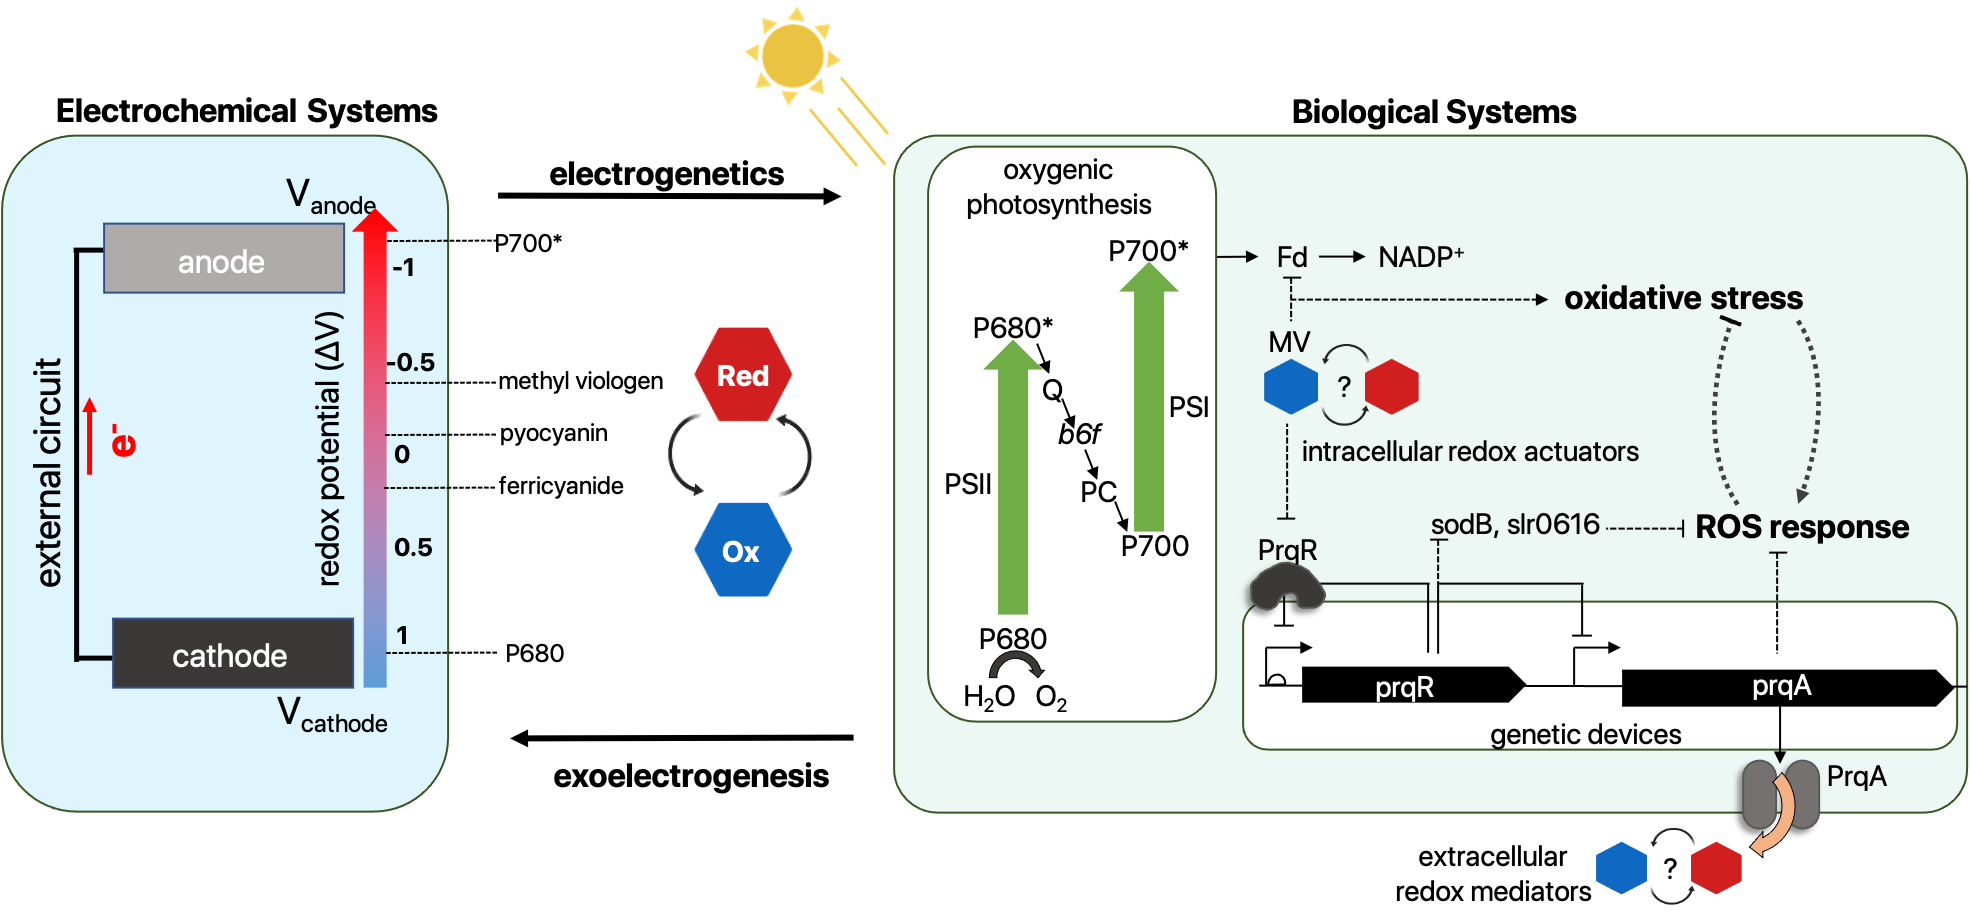
\includegraphics[width=\hsize]{figs/fintro.png}
    \caption{Electrochemical devices like the voltaic cell shown in blue are systems that can use electrical energy to catalyse redox reactions (allowing electrogenetic control) or, inversely, generating electricity from chemical reactions (exploiting exoelectrogenic bacteria to generate electricity). By imposing a potential energy difference between cathode and anodes, these devices can selectively catalyse oxidation or reduction of redox-mediator compounds (e.g. pyocyanin, methyl viologen etc...) according to their standard redox potential. Identifying redox-mediators that can regulate the activity of genetically-encoded regulators (without interfering with the host photosynthetic redox reactions),  allows to investigate how cells can transduce environmental redox signals into biological responses. This project will focus on a specific genetic regulatory system formed by the prqRA operon, which encodes a putative redox-sensitive repressor and an uncharacterised transmembrane protein with predicted transport activity of redox compounds. Abbreviations= PSII: Photosystem II; P680: Photosystem II primary donor pigment; P700: Photosystem I primary donor pigment; PSI: Photosystem II; Q: quinol; b6f: cytochrome b6f; PC: plastocyanin; Fd: ferredoxin; MV: methyl viologen; ROS: reactive-oxygen-species. V: electrode potential.}
\end{figure}

\subsection{Aims and Research Questions}
In summary, the general scope of the project is to develop a framework to understand and characterise a specific genetic circuit (the prqRA operon) that regulates redox signal transduction in a model cyanobacterium often employed in bioelectrochemical systems. 
The aim is to understand the bioelectrochemical mechanisms that these photosynthetic bacteria have evolved to respond to exogenous redox stresses.
The main hypothesis that underlies this project is that when bacteria are employed in bioelectrochemical systems they may experience both direct and indirect oxidative stresses (e.g. ROS-generating redox mediators, externally-applied oxidative electrode potentials), resulting in upregulation of ROS-quenching adaptive responses (e.g. overexpression of redox-sensitive transcriptional regulators and transmembrane proteins exporting redox-active byproducts). 
Whereas evidence supporting this hypothesis is available for other bacteria, such as the heterotrophic \textit{Pseudomonas} \citep{Nikel2021} and the chemolitotrophic \textit{Geobacter} species \citep{Levar2017}, its validity and biochemical details still need to be investigated in photosynthetic prokaryotes. 
Understanding this is of particular biotechnological importance, as it could permit to rationally engineer redox-tolerant cyanobacterial strains with increased exoelectrogenic activity and synthetic electrogenetic plasmids that can operate in oxidative conditions.
In order to achieve these goals, this PhD project aims to answer the three big questions listed below. For each of these questions, this study outlines a workflow to solve their more specific and experimentally-answerable subquestions.   

\begin{enumerate}
    \item What are the mechanisms and functions of redox transcriptional repression by PrqR ?
    \begin{itemize}
        \item Is it possible to generate markerless mutations in the prqRA operon in \textit{Synechocystis} cells using Cas12a-mediated gene editing techniques?
        \item How does the genetic expression from the prqRA operon in mutant strains compare with wild-type cells, in different redox environments (applied external bias potential and after incubation with ROS-generating redox mediators)?
        \item Do the $\Delta$prqR mutants show a growth advantage compared to WT, $\Delta$prqA and $\Delta$prqRA strains in conditions promoting oxidative stress ? 
        \item Can the phenotypes of the mutants be restored to wild-type when mutant strains are transformed with their respective complementation plasmids?
    \end{itemize}
    \item Is it possible to repurpose the redox-sensitive prqRA operon to construct reporter plasmids inducible by externally applied redox signals?
        \begin{itemize}
            \item Does the fluorescence intensity measured in cyanobacteria transformed with genetic construct expressing fluorescent reporter proteins under the control of the $P_{prqR}$ promoter show a sigmoidal response to the concentration of ROS-generating exogenously-added ligands ?
            \item Can these redox-active mediators be selectively oxidised or reduced by an external electrode with a midpoint potential orthogonal to those of key photosynthetic reactions?
        \end{itemize}
    \item Is it possible to genetically engineer strains of cyanobacteria with increased robustness to oxidative perturbations in order to increase their exoelectrogenic activity ?
      \begin{itemize}
            \item How does the exoelectrogenic activity of $\Delta$prqR, $\Delta$prqA and $\Delta$prqRA mutants compare to wild-type \textit{Synechocystis} cells?
    \end{itemize}    
\end{enumerate}


\section{Experimental Design}
To address the questions above this project employs two complementary experimental strategies. First, \textit{Synechocystis sp.} PCC 6803 cells will be genetically engineered to obtain redox-sensitive mutant strains with deletion in prqR, prqA and the whole prqRA operon, as listed in Table \ref{table:strains}. Then, these mutant strains will be used as hosts to characterise the expression of synthetic reporter plasmids (Figure \ref{fig:reporters}) containing a fluorescent reporter protein cloned downstream of the redox-sensitive $P_{prqR}$ promoter, which regulates the expression of the prqRA operon. A theoretical framework to mathematically model the gene expression dynamics from the prqRA operon will be also employed to guide the experimental design and to interpret the results from the experimental characterisation of the reporter plasmids.


\subsection{Rationale and Strategy to Generate Mutant Cyanobacteria}
All the mutants described in this study are derived from a mother culture of wild-type \textit{Synechocystis sp.} PCC 6803, which was obtained from a glycerol stock in the Howe lab (David Lea-Smith). These cultures were propagated in standard BG-11 medium in Erlenmeyer flasks shaking at 100 rpm, 30 $^{\circ}$C and 40 $\mu$mol photons $m^{\UTF{2013}2} s^{\UTF{2013}1}$
To generate the knock-out mutants, custom plasmids for CRISPR-mediated genome editing have been constructed, as summarised in Figure \ref{fig:kostra}. A CRISPR-based approach has been chosen because it can generate markerless genome modification with a higher efficiency and in a shorter amount of time compared to the classic homologous recombination method \citep{Behler2018}. In addition, another PhD student in the Howe lab is developing a similar strategy for CRISPR interference experiments and therefore most of the level 1 CRISPR expression cassettes were already available in the lab. Since the Cas12a protein has been previously shown to be able to work in this host \citep{Ungerer2016}, this has been chosen as endonuclease for the genome editing plasmids developed during this study. These plasmids have been assembled with a standardised architecture to enable rapid and modular construction of novel knock-out constructs targeting different genes, which could be helpful for future experiments. Detailed information on the genetic parts included in these plasmids are available in the supplementary information. Briefly, these constructs are derived from the backbone pCAT.011, a mid-copy number replicative plasmid that can propagate in both \textit{E. coli} and a broad range of cyanobacterial hosts and contain three inserts in the multiple cloning site. Position 1 harbours the coding sequence for Cas12a under the control of constitutive Anderson promoters  of increasing strengths. In position 2, under the control of the strongest constitutive promoter (J23119), there is the sequence encoding the guide RNAs with a 23 bp long spacer region targeting the Cas12a to the genomic locus to be cut (at a location of 18\UTF{2013}19 bases from the 3′ end of the PAM sequence 5′-TTTV-3′). Finally, position 3 is dedicated to the homology repair templates, $\approx$ 250 bp long DNA sequences homologous to the upstream and downstream regions flanking the cut site and encoding the mutation of interest.

\begin{figure}[H]
    \centering
    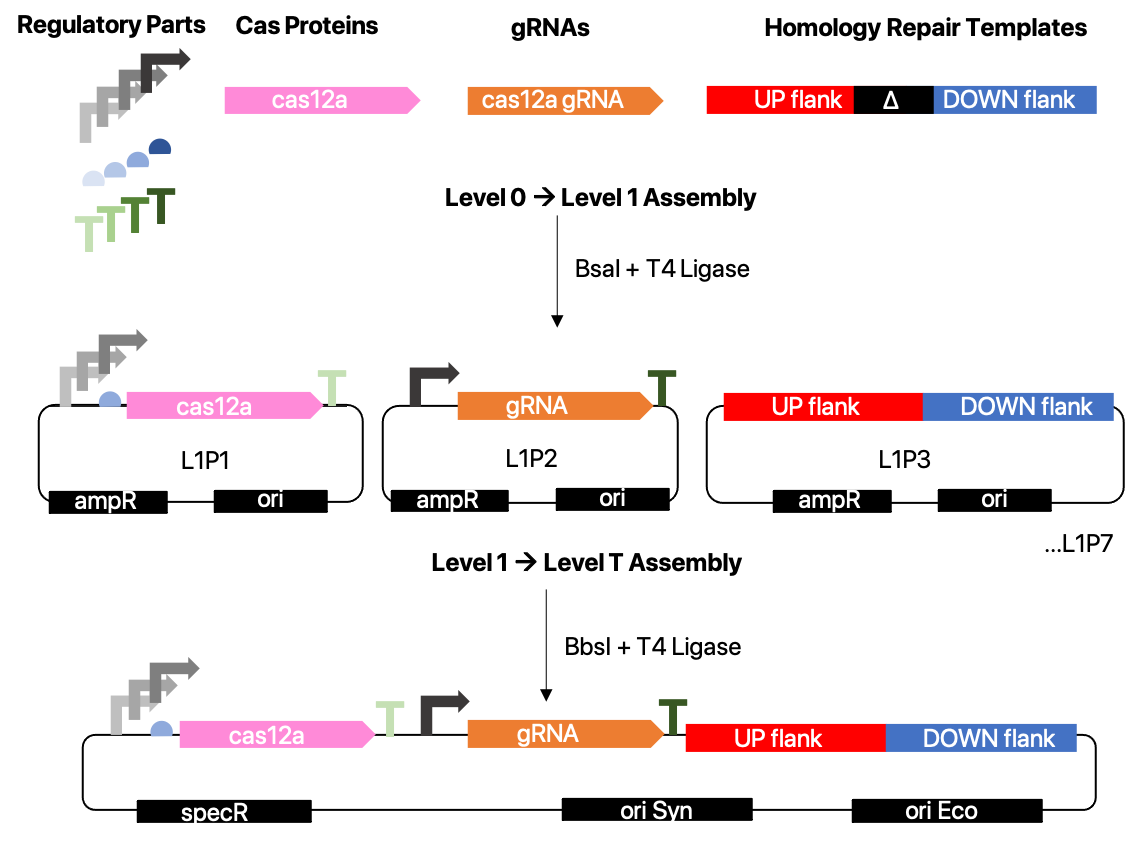
\includegraphics[width=0.8\hsize]{figs/KOstrategy.png}
    \caption{Diagram of the cloning strategy used to construct the knock-out constructs for this study. Regulatory parts like promoters (bent arrows), ribosome binding sites (filled half-circles), terminators (T) and the acceptor backbones have been taken from the CyanoGate and Plant MoClo toolboxes (\citealt{Vasudevan2019};\citealt{Engler2014}). The CRISPR expression cassettes kindly given to me by Joshua Lawrence. The gRNAs and homology repair templates have been cloned during this study from the genome of \textit{Synechocystis sp.} PCC 6803 via oligo annealing and PCR amplification respectively. The modular nature of this cloning strategy enables to assemble level 0 DNA parts into genetic devices with only 2 one-pot reactions, and is compatible with multipart, combinatorial assembly of DNA sequences with standardised overhangs.
}
\label{fig:kostra}
\end{figure}

\subsection{Constructing P\textsubscript{prqR} Reporter Plasmids}
To quantify genetic expression from the $P_{prqR}$ promoter, reporter plasmids have been constructed by cloning the $P_{prqR}$ sequence upstream of the enhanced Yellow Fluorescent reporter Protein (eYFP). The promoter sequence was identified by bioinformatic analysis (Fig. \ref{fig:promoteranal}) and was cloned by annealing and extension of oligonucleotides primers. Different versions and controls for these devices have been constructed. A positive control harbours eYFP upstream of J23119, a very strong, constitutive promoter commonly used as reference in synthetic biology. A negative control was initially devised as the backbone plasmid with no eYFP added. Following discussions with members of my postgraduate panel, it was suggested instead to construct a plasmid containing eYFP and a randomised promoter sequence upstream, to account for leakiness of transcription. A plasmid of this kind (pAST.43) was therefore constructed. Two versions for P$_{prqR}$ reporter plasmids have been designed. The first one (pAST.40) is a synthetic version of the prqRA operon, in which the native downstream gene (prqA) was replaced by eYFP. This device will be transformed in \textit{Synechocystis} cells with the genomic prqR knocked-out ($\Delta$prqR) and in \textit{E. coli} to rapidly screen putative PrqR ligands with a plate reader. The second version (pAST.41), contains the eYFP coding sequence downstream of the P$_{prqR}$ promoter.

\begin{figure}[H]
    \centering
    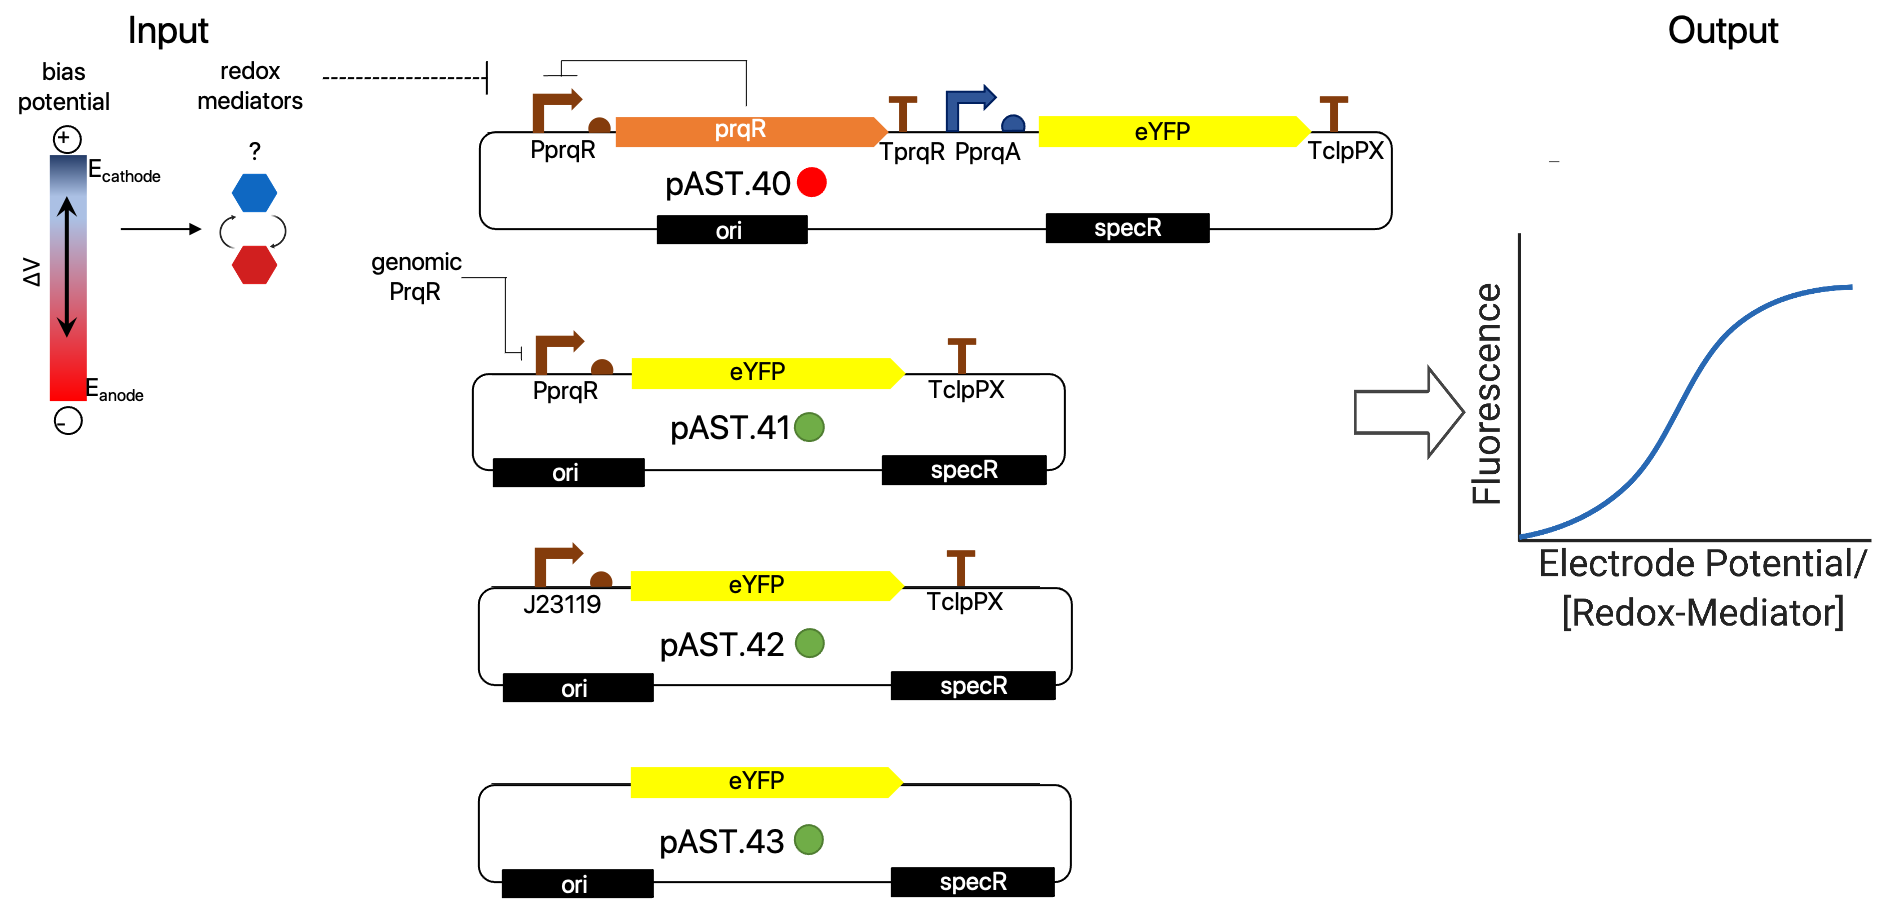
\includegraphics[width=\hsize]{figs/reporters.png}
    \caption{Fluorescent reporter devices to quantify genetic expression from $P_{prqR}$.}
    \label{fig:reporters}
\end{figure}
\newpage
\subsection{DNA Assembly of Plasmids}
All the plasmids generated in this study were assembled using a Golden Gate strategy with MoClo standards developed for synthetic biology in cyanobacteria \citep{Vasudevan2019}. This strategy was used because of its high efficiency, the possibility to perform the restriction and ligation step in a one-pot reaction and the availability of standardised overhangs compatible with other cloning systems \citep{Weber2011}. All the level 0 and 1 and T plasmids were subcloned in  chemically competent \textit{E. coli} cells, propagated at 37$\circ$C in LB media with their respective antibiotics (60 $\mu$g/mL spectinomycin for level 0 and T, 100 $\mu$g/mL carbenicillin for level 1). All the level 0 DNA parts were cloned from \textit{Synechocystis} genomes using primers listed in Table \ref{table:primers} and with standard PCR conditions. Parts shorter than 100 bp (e.g. promoters and gRNAs) were assembled by annealing synthetic oligonucleotides in a PCR thermocycler, as explained in Section \ref{sec:Annealing}. The level T plasmids were transformed in WT \textit{Synechocystis sp.} cells. Briefly, every DNA assembly reaction was carried out in PCR tubes with 1$\mu$l of restriction enzyme (BbsI-HF for level 0 and T, BsaI-HF for level T; both from 20,000 units/ml stocks from NEB), 1 $\mu$l of T4 DNA ligase (from 5u/$mu$l stock, \href{https://www.thermofisher.com/order/catalog/product/EL0011#/EL0011}{ThermoFisher}), 2$\mu$l ATP (from 100 mM stock), 2$\mu$l BSA (from 20 ml/ml stock, \href{https://www.thermofisher.com/order/catalog/product/B14?uk&en#/B14?uk&en}{ThermoFisher}), 2$\mu$l buffer G (from 10x stock, \href{https://www.thermofisher.com/order/catalog/product/BG5?uk&en#/BG5?uk&en}{ThermoFisher}), 0.75 ng of purified backbone plasmid and a 2:1 insert to backbone ratio. These tubes were then placed in a thermocycler programmed to perform 30 cycles at 37$^{\circ}$C (to activate restriction enzyme) and 16$^{\circ}$C (to activate T4 DNA ligase) of 5 min each. The assembly reaction mixtures were then added with 10 $\mu$l of 5x KCM to 40 $\mu$l of chemically competent cells (\href{https://international.neb.com/products/c2987-neb-5-alpha-competent-e-coli-high-efficiency}{NEB 5-alpha}) in sterile PCR tubes. Heat-shock was performed in a PCR thermocycler according to the instructions of the competent cell manufacturer. The transformation reaction mixtures were spreaded onto LB plates supplemented with 1.5 \% agar, 100mM IPTG (from 1000x stock), 20 mg/ml X-Gal (from 1000x stock) and the appropriate antibiotics. After overnight incubation at 37$^{\circ}$, white colonies were picked from plates and grown overnight in liquid LB medium (with respective antibiotic). After 16-24 hours, cultures were centrifuged and their plasmid DNA extracted with a Miniprep kit (\href{https://www.thermofisher.com/order/catalog/product/K0503?ICID=cvc-pdna-miniprep-c1t1#/K0503?ICID=cvc-pdna-miniprep-c1t1}{ThermoFisher}). The concentration and purity of the purified plasmids was measured with a Nanodrop and then sent for Sanger DNA sequencing. 


\subsection{Natural Transformation of \textit{Synechocystis sp.} PCC 6803}
\label{sec:transf}
After having assembled the knock-out and reporter plasmids in \textit{E. coli} these plasmids were sequenced and transformed into wild-type \textit{Synechocystis sp.} PCC 6803 cells following the natural transformation protocol described by \cite{Pope2020}.
Three separate colonies \textit{Synechocystis} were picked from a BG-11 plate, previously streaked with an axenic culture from a glycerol stock in the lab. These colonies were inoculated in 10 ml of low-phosphate liquid BG-11 medium without glucose, and grown under 40 $\mu$mol photons $m^{\UTF{2013}2} s^{\UTF{2013}1}$ of fluorescent white light, shaking at 100 rpm at 31$\circ$C in air for $\approx$ 7 days. 
Then 1 mL of cells was collected by centrifugation in a 2 ml Eppendorf tube, washed twice in no-phosphate BG-11 and resuspended in 1 ml of no-phosphate BG-11 to give a final OD740 of 1. Cells were collected again by centrifugation and 1 $\mu$g of plasmid DNA was added to the tube. In the wells of a 12-well microplate, no-phosphate BG-11 was added to a final volume of 100 $\mu$l. Cells were resuspended and the microplate was sealed with parafilm and left in  40 $\mu$mol photons $m^{\UTF{2013}2} s^{\UTF{2013}1}$) in 30$^{\circ}$C for 6 h, shaking at 100 rpm. After 6 h, 10 $\mu$l of cell suspension was spotted onto a no-phosphate BG-11 agar plate. The plate was incubated at 30$^{\circ}$C under 40 $\mu$mol photons $m^{\UTF{2013}2} s^{\UTF{2013}1}$ of white light for 24 h. This plate is used as a positive control to calculate the maximum number of colonies appearing on plates prior to the addition of negative selection.
After 24 h the liquid cultures in the wells of the microplate were centrifuged and re-suspended again in 100 $\mu$l of no-phosphate BG-11 containing the negative selection marker (spectinomycin) at a final concentration of 60 $\mu$g/ml.
After 24 h, 10 $\mu$l of this cell suspension was  spotted onto a no-phosphate BG-11 agar plate containing spectinomycin) at a final concentration of 60 $\mu$g/ml. This plate was incubated at 30$^{\circ}$C under 40 $\mu$mol photons $m^{\UTF{2013}2} s^{\UTF{2013}1}$ of white light until the appearance of colonies. Cells that have been successfully transformed with plasmids containing spectinomycin-resistant should grow on this plate. By dividing the number of colony forming units on this plate by the number of colonies growing in the positive control plate (no negative selection), it is possible to estimate the transformation efficiency for this experiment.

\section{Results}
\subsection{Assembly of Knock-Out and Reporter Plasmids}

All the assembled genetic parts have been subcloned in \textit{E. coli}. After picking and extracting the plasmid content from the white colonies growing in the transformation plates, the DNA sequences have been validated by aligning the Sanger sequencing reads with the \textit{in silico} designs of the constructs. The tables below summarise these results and show the progress of the cloning strategy performed since the start of this project. 

\begin{table}[H]
\centering
\begin{tabular}{|c|c|c|c|c|}
\hline
\textbf{Part} & \textbf{Backbone} & \textbf{Insert} & \textbf{Type} & \textbf{DNA Seq} \\ \hline
pAS0.1 & pICH41308 & prqR & PrqR coding sequence & \cellcolor[HTML]{FFFE65} \href{https://scaralbi.github.io/assets/dna/L0/2020-11-13_D01_ASAS01ASP1-alignment.pdf}{ASAS01ASP1} \\ \hline
pAS0.2 & pICH41308 & prqA & PrqA coding sequence & \cellcolor[HTML]{32CB00} \href{https://scaralbi.github.io/assets/dna/L0/2020-10-29_E10_JLPAS02SP1-alignment.pdf}{JLPAS02SP1} \\ \hline
pAS0.5 & pICH41331 & prqRA HRT & homology repair template ($\Delta$prqRA) & \cellcolor[HTML]{32CB00} \href{https://scaralbi.github.io/assets/dna/L0/2020-10-29_E10_JLPAS02SP1-alignment.pdf}{ASPAS5SP1} \\ \hline
pAS0.6 & pICH41295 & $P_{prqR}$ & native promoter + RBS & \cellcolor[HTML]{32CB00} \href{https://scaralbi.github.io/assets/dna/L0/2020-11-03_G01_ASASO6ASP1-alignment.pdf}{ASASO6ASP1} \\ \hline
pAS0.7 & pICH42120 & gRNA-prqR & cas12a gRNA & \cellcolor[HTML]{32CB00} \href{https://scaralbi.github.io/assets/dna/L0/2020-07-28_H07_AS7SP1-alignment.pdf}{AS7SP1} \\ \hline
pAS0.8 & pICH41331 & prqR HRT & homology repair template ($\Delta$prqR)  & \cellcolor[HTML]{32CB00} \href{https://scaralbi.github.io/assets/dna/L0/2020-07-30_E11_ASPAS8SP1-2020-07-30_E11_ASPAS8SP1ab1-alignment.pdf}{ASPAS8SP1} \\ \hline
pAS0.10 & pICH42120 & gRNA prqA & cas12a gRNA & \cellcolor[HTML]{32CB00} \href{https://scaralbi.github.io/assets/dna/L0/2020-09-07_B02_ASAS010SP1-alignment.pdf}{AS10SP1} \\ \hline
pAS0.11 & pICH41331 & prqA HRT & homology repair template ($\Delta$prqA)  & \cellcolor[HTML]{32CB00} \href{https://scaralbi.github.io/assets/dna/L0/2020-11-03_A02_ASASO11ASP1-alignment.pdf}{ASASO11ASP1} \\ \hline
pAS0.12 & pICH41295 & PprqA & native promoter TSS & \cellcolor[HTML]{32CB00} \href{https://scaralbi.github.io/assets/dna/L0/2020-11-13_H01_ASAS012ASP1-alignment.pdf}{ASAS012ASP1} \\ \hline
pAS0.13 & pICH41276 & TprqR & native terminator & \cellcolor[HTML]{32CB00} \href{https://scaralbi.github.io/assets/dna/L0/2020-11-03_E01_ASASO13ASP1-alignment.pdf}{ASASO13ASP1} \\ \hline
pAS0.14 & pICH41308 & mScarletI & reporter coding sequence & \cellcolor[HTML]{32CB00} \href{https://scaralbi.github.io/assets/dna/L0/2020-11-16_G09_ASASO14BSP1-alignment.pdf}{ASASO14BSP1} \\ \hline
\end{tabular}
\caption{List of level 0 plasmids. Inserts are cut out with restriction enzyme BsaI. Positive selection: spectinomycin. Green: part has been been succesfully assembled (DNA sequencing alignment available in hyperlink). Yellow: part has been assembled but contains undesired mutations. Red: part has not been assembled yet.}
\label{table:level0}
\end{table}

The majority of the required level 0 parts (which contain basic genetic units such as coding and regulatory sequences) have been successfully assembled. Only the coding sequence for the the PrqR protein needs to be reassembled, as it contains a BbsI recognition site that needs to be domesticated.

\begin{table}[H]
\centering
\begin{tabular}{|l|l|c|c|c|c|}
\hline
\multicolumn{1}{|c|}{\textbf{Part}} & \multicolumn{1}{c|}{\textbf{Backbone}} & \textbf{Insert(s)} & \textbf{Type} & \textbf{DNA Seq} \\ \hline
pAS1.1 & L1P3 & pAS0.8 & prqR HRT & \cellcolor[HTML]{32CB00} \href{https://scaralbi.github.io/assets/dna/L1/2020-09-07_E02_ASAS112SP3-2020-09-07_E02_ASAS112SP3ab1-alignment.pdf}{AS112SP3} \\ \hline
pAS1.2 & L1P3 & pAS0.5 & prqRA HRT & \cellcolor[HTML]{32CB00} \href{https://scaralbi.github.io/assets/dna/L1/2020-09-07_F02_ASAS12SP3-2020-09-07_F02_ASAS12SP3ab1-alignment.pdf}{AS121SP3} \\ \hline
pAS1.3 & L1P2 & J23108$_{TSS}$+pAS0.7+T$_{clpPX}$ & prqR gRNA1 & \cellcolor[HTML]{32CB00} \href{https://scaralbi.github.io/assets/dna/L1/2020-09-07_G02_ASAS131SP3-2020-09-07_G02_ASAS131SP3ab1-alignment.pdf}{AS131SP3} \\ \hline
pAS1.4 & L1P2 & J23119$_{TSS}$+pAS0.7+T$_{clpPX}$ & prqR gRNA2 & \cellcolor[HTML]{32CB00} \href{https://scaralbi.github.io/assets/dna/L1/2020-11-19_F08_ASAS14BSP3-alignment.pdf}{AS14BSP3} \\ \hline
pAS1.6 & L1P3 & pAS0.11 & prqA HRT  & \cellcolor[HTML]{32CB00} \href{https://scaralbi.github.io/assets/dna/L1/2020-11-19_B09_ASAS16BSP3-alignment.pdf}{AS16BSP3} \\ \hline
pAS1.7 & L1P1 & pAS0.6+pAS0.1+pAS0.13 & prqR  & \cellcolor[HTML]{32CB00} \href{https://scaralbi.github.io/assets/dna/L1/2020-11-19_D09_ASAS17BSP3-alignment.pdf}{AS17BSP3}  \\ \hline
pAS1.8 & L1P2 & J23108$_{TSS}$+pAS0.10+T$_{clpPX}$ & prqA gRNA1  & \cellcolor[HTML]{32CB00} \href{https://scaralbi.github.io/assets/dna/L1/2020-11-13_E02_ASAS18BSP4-alignment.pdf}{AS18BSP4}  \\ \hline
pAS1.9 & L1P2 & J23119$_{TSS}$+pAS0.10+T$_{clpPX}$ & prqA gRNA2  & \cellcolor[HTML]{FE0000}  \\ \hline
pAS1.10 & L1P1 & J23119$_{v02}$+pAS0.1+T$_{clpPX}$ & PrqR overexpression & \cellcolor[HTML]{FE0000}  \\ \hline
pAS1.11 & L1P2 & pAS0.12+eYFP+T$_{clpPX}$ & $P_{prqA}$ eYFP reporter  & \cellcolor[HTML]{32CB00} \href{https://scaralbi.github.io/assets/dna/L1/2020-11-19_B10_ASAS111BSP3-alignment.pdf}{AS111BSP3} \\ \hline
pAS1.13 & L1P1 & J23119$_{v02}$+eYFP+T$_{clpPX}$ & eYFP +ve control  & \cellcolor[HTML]{32CB00} \href{https://scaralbi.github.io/assets/dna/L1/2020-11-19_F10_ASAS113BSP3-alignment.pdf}{AS113BSP3} \\ \hline
pAS1.14 & L1P1 & pAS0.6+eYFP+T$_{clpPX}$ & $P_{prqR}$-eYFP reporter & \cellcolor[HTML]{32CB00} \href{https://scaralbi.github.io/assets/dna/L1/2020-12-01_E06_ASJL114ASP4-alignment.pdf}{JL114ASP4} \\ \hline
pAS1.15 & L1P1 & \multicolumn{1}{l|}{J23119$_{v02}$+pAS0.14+T$_{clpPX}$} & mScarletI +ve control & \cellcolor[HTML]{32CB00} \href{https://scaralbi.github.io/assets/dna/L1/2020-12-15_F07_JLJL115ASP4-alignment.pdf}{JL115ASP4} \\ \hline
\end{tabular}
\caption{List of level 1 plasmids. Inserts are cut out with restriction enzyme BbsI. Positive selection: ampicillin/carbenicillin. Green: part has been been succesfully assembled (DNA sequencing alignment available in hyperlink). Yellow: part has been assembled but contains undesired mutations. Red: part has not been assembled yet.}
\label{table:level1}
\end{table}

The majority of the required level 1 constructs (which encode expression cassettes and specify the position of these parts in the final level T vectors) have also been successfully validated by DNA sequencing. One gRNA expression unit (under control of strong J23119 promoter) and the PrqR overexpression construct (which required the correct PrqR coding sequence) still need to be reassembled.

\begin{table}[H]
\centering
\begin{tabular}{|l|l|l|l|l|}
\hline
\multicolumn{1}{|c|}{\textbf{Part}} & \multicolumn{1}{c|}{\textbf{Backbone}} & \multicolumn{1}{c|}{\textbf{Insert(s)}} & \multicolumn{1}{c|}{\textbf{Type}} & \multicolumn{1}{c|}{\textbf{DNA Seq}} \\ \hline
pAST.000 & pCAT.011 & pJML1.017+pAS1.4+pAS1.1 & $\Delta$prqR J23105-cas12a & \cellcolor[HTML]{FE0000}{\color[HTML]{FE0000} } \\ \hline
pAST.001 & pCAT.011 & pJML1.016+pAS1.4+pAS1.1 & $\Delta$prqR J23114-cas12a  & \cellcolor[HTML]{32CB00}{\color[HTML]{000000} \href{https://scaralbi.github.io/assets/dna/LT/2020-12-04_G02_ASAST15BSPTF-alignment.pdf}{T1ASPTF}} \\ \hline
pAST.002 & pCAT.011 & pJML1.015+pAS1.4+pAS1.1 & $\Delta$prqR J23117-cas12a  & \cellcolor[HTML]{FE0000} \\ \hline
pAST.010 & pCAT.011 & pJML1.017+pAS1.3+pAS1.2 & $\Delta$prqRA J23105-cas12a & \cellcolor[HTML]{32CB00}T15BASTF \\ \hline
pAST.011 & pCAT.011 & pJML1.016+pAS1.3+pAS1.2 & $\Delta$prqRA J23114-cas12a  & \cellcolor[HTML]{FE0000} \\ \hline
pAST.012 & pCAT.011 & pJML1.015+pAS1.3+pAS1.2 & $\Delta$prqRA J23117-cas12a& \cellcolor[HTML]{FE0000} \\ \hline
pAST.020 & pCAT.011 & pJML1.017+pAS1.8+pAS1.6 & $\Delta$prqA J23105-cas12a & \cellcolor[HTML]{FE0000} \\ \hline
pAST.021 & pCAT.011 & pJML1.016+pAS1.8+pAS1.6 & $\Delta$prqA J23114-cas12a & \cellcolor[HTML]{32CB00}{\color[HTML]{000000} T21ASTF} \\ \hline
pAST.022 & pCAT.011 & pJML1.015+pAS1.8+pAS1.6 & $\Delta$prqA J23117-cas12a & \cellcolor[HTML]{FE0000} \\ \hline
pAST.040 & pCAT.011 & pAS1.7 + pAS1.11 & prqRA reporter1 & \cellcolor[HTML]{FE0000} \\ \hline
pAST.041 & pCAT.011 & pAS1.14 & prqRA reporter 2 & \cellcolor[HTML]{32CB00}\href{https://scaralbi.github.io/assets/dna/LT/2020-12-10_A10_AST41DSPTF-2020-12-10_G09_AST41BSPTF-2020-12-10_F09_AST41ASPTF-2020-12-10_H09_AST41CSPTF-alignment.pdf}{T41STF} \\ \hline
pAST.042 & pCAT.011 & pAS1.13 & eYFP +ve control & \cellcolor[HTML]{32CB00}\href{https://scaralbi.github.io/assets/dna/LT/2020-12-10_B10_AST42ASPTF-alignment.pdf}{T42STF} \\ \hline
\end{tabular}
\caption{List of level T plasmids. Do not contain BbsI or BsaI sites. Positive selection: spectinomycin. Green: part has been been succesfully assembled (DNA sequencing alignment available in hyperlink). Yellow: part has been assembled but contains undesired mutations. Red: part has not been assembled yet.}
\label{table:levelT}
\end{table}

With regards to the knock-out level T plasmids,  at least one version for every type of knock-out strain ($\Delta$prqR, $\Delta$prqA, $\Delta$prqRA ) has been assembled. Additional versions of these constructs with cas12a under the control of other promoters still need to be re-assembled. For the reporter plasmids, 2 out of the 3 constructs required have been validated. The remaining plasmid requires the correct version of the prqR coding sequence, which has not been domesticated yet.

\subsection{Transformation and Selection of Mutants}
\label{sec:trans}
After validating the sequences of the level T plasmids, some of those that have been successfully assembled have been transformed in wild-type \textit{Synechocystis sp.} PCC 6803 cells according to the natural transformation protocol described in Section \ref{sec:transf}. The backbone plasmid (containing the spectinomycin resistance gene already validated to work in \textit{Synechocystis sp.} PCC 6803 by \citep{Vasudevan2019} have been transformed as positive controls. For the negative control, no plasmid DNA was added. Figure \ref{fig:transplate} shows the outcome of this experiment for three biological replicates of WT \textit{Synechocystis sp. PCC} transformed with the plasmids labelled on the left and spotted (at different dilutions) on BG11 plates containing specinomycin as selection marker.

\begin{figure}[H]
    \centering
    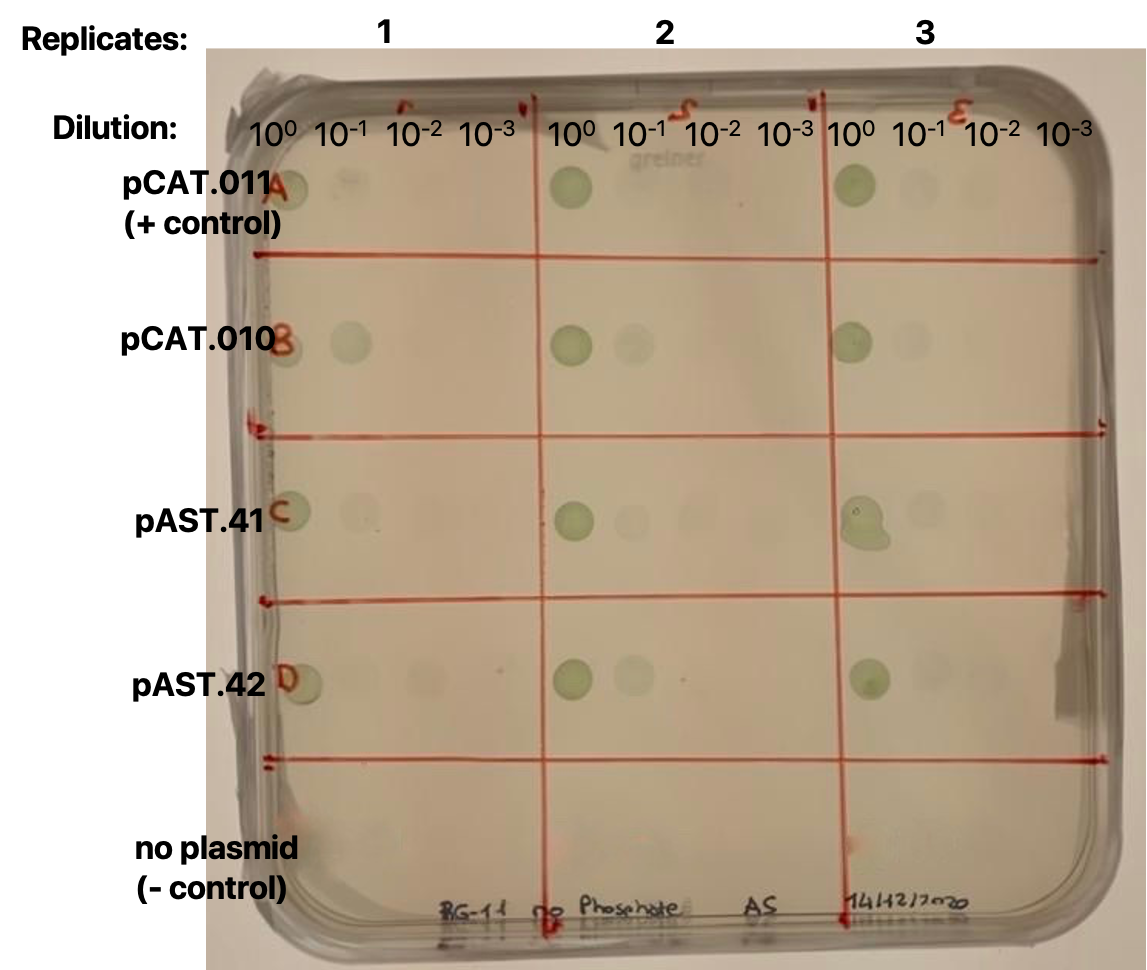
\includegraphics[width=0.6\hsize]{figs/trans.png}
    \caption{BG-11 + Spectinomycin plate spotted with cultures of \textit{Synechocystis sp.} PCC 6803. These results do not prove that the colonies growing on these plates contain the desired genotypes, but only that the transformation protocol and antibiotic selection employed work.}
    \label{fig:transplate}
\end{figure}


\subsection{Characterisation of Reporter Constructs}
\label{sec:charactreporter}
As shown in Table \ref{table:levelT}, most of the sequences of the reporter constructs have been succesfully validated by DNA sequencing. Before transformation in \textit{Synechocystis sp.} PCC 6803, an experiment was performed to characterise these plasmids in \textit{E. coli}. Constructs that express in \textit{E. coli} also usually work in \textit{Synechocystis sp. PCC} 6803 (although with different dynamic profiles). With this assumption, the reason behind this experiment was to prove that these constructs (that have been genotypically validated) also resulted in the phenotypic emission of a fluorescent signals characteristic of eYFP. Although their DNA sequences were correct, given the stochastic nature of biological systems it seemed cautious not to take this for granted. Using \textit{E. coli} it was possible to rapidly solve this doubt using a plate reader.  This experiment confirms that the constructs encoding eYFP resulted in the emission of a fluorescent signal detected at 527 nm that is characteristic of eYFP (Figure \ref{fig:platereader}). 

\begin{figure}[H]
    \centering
    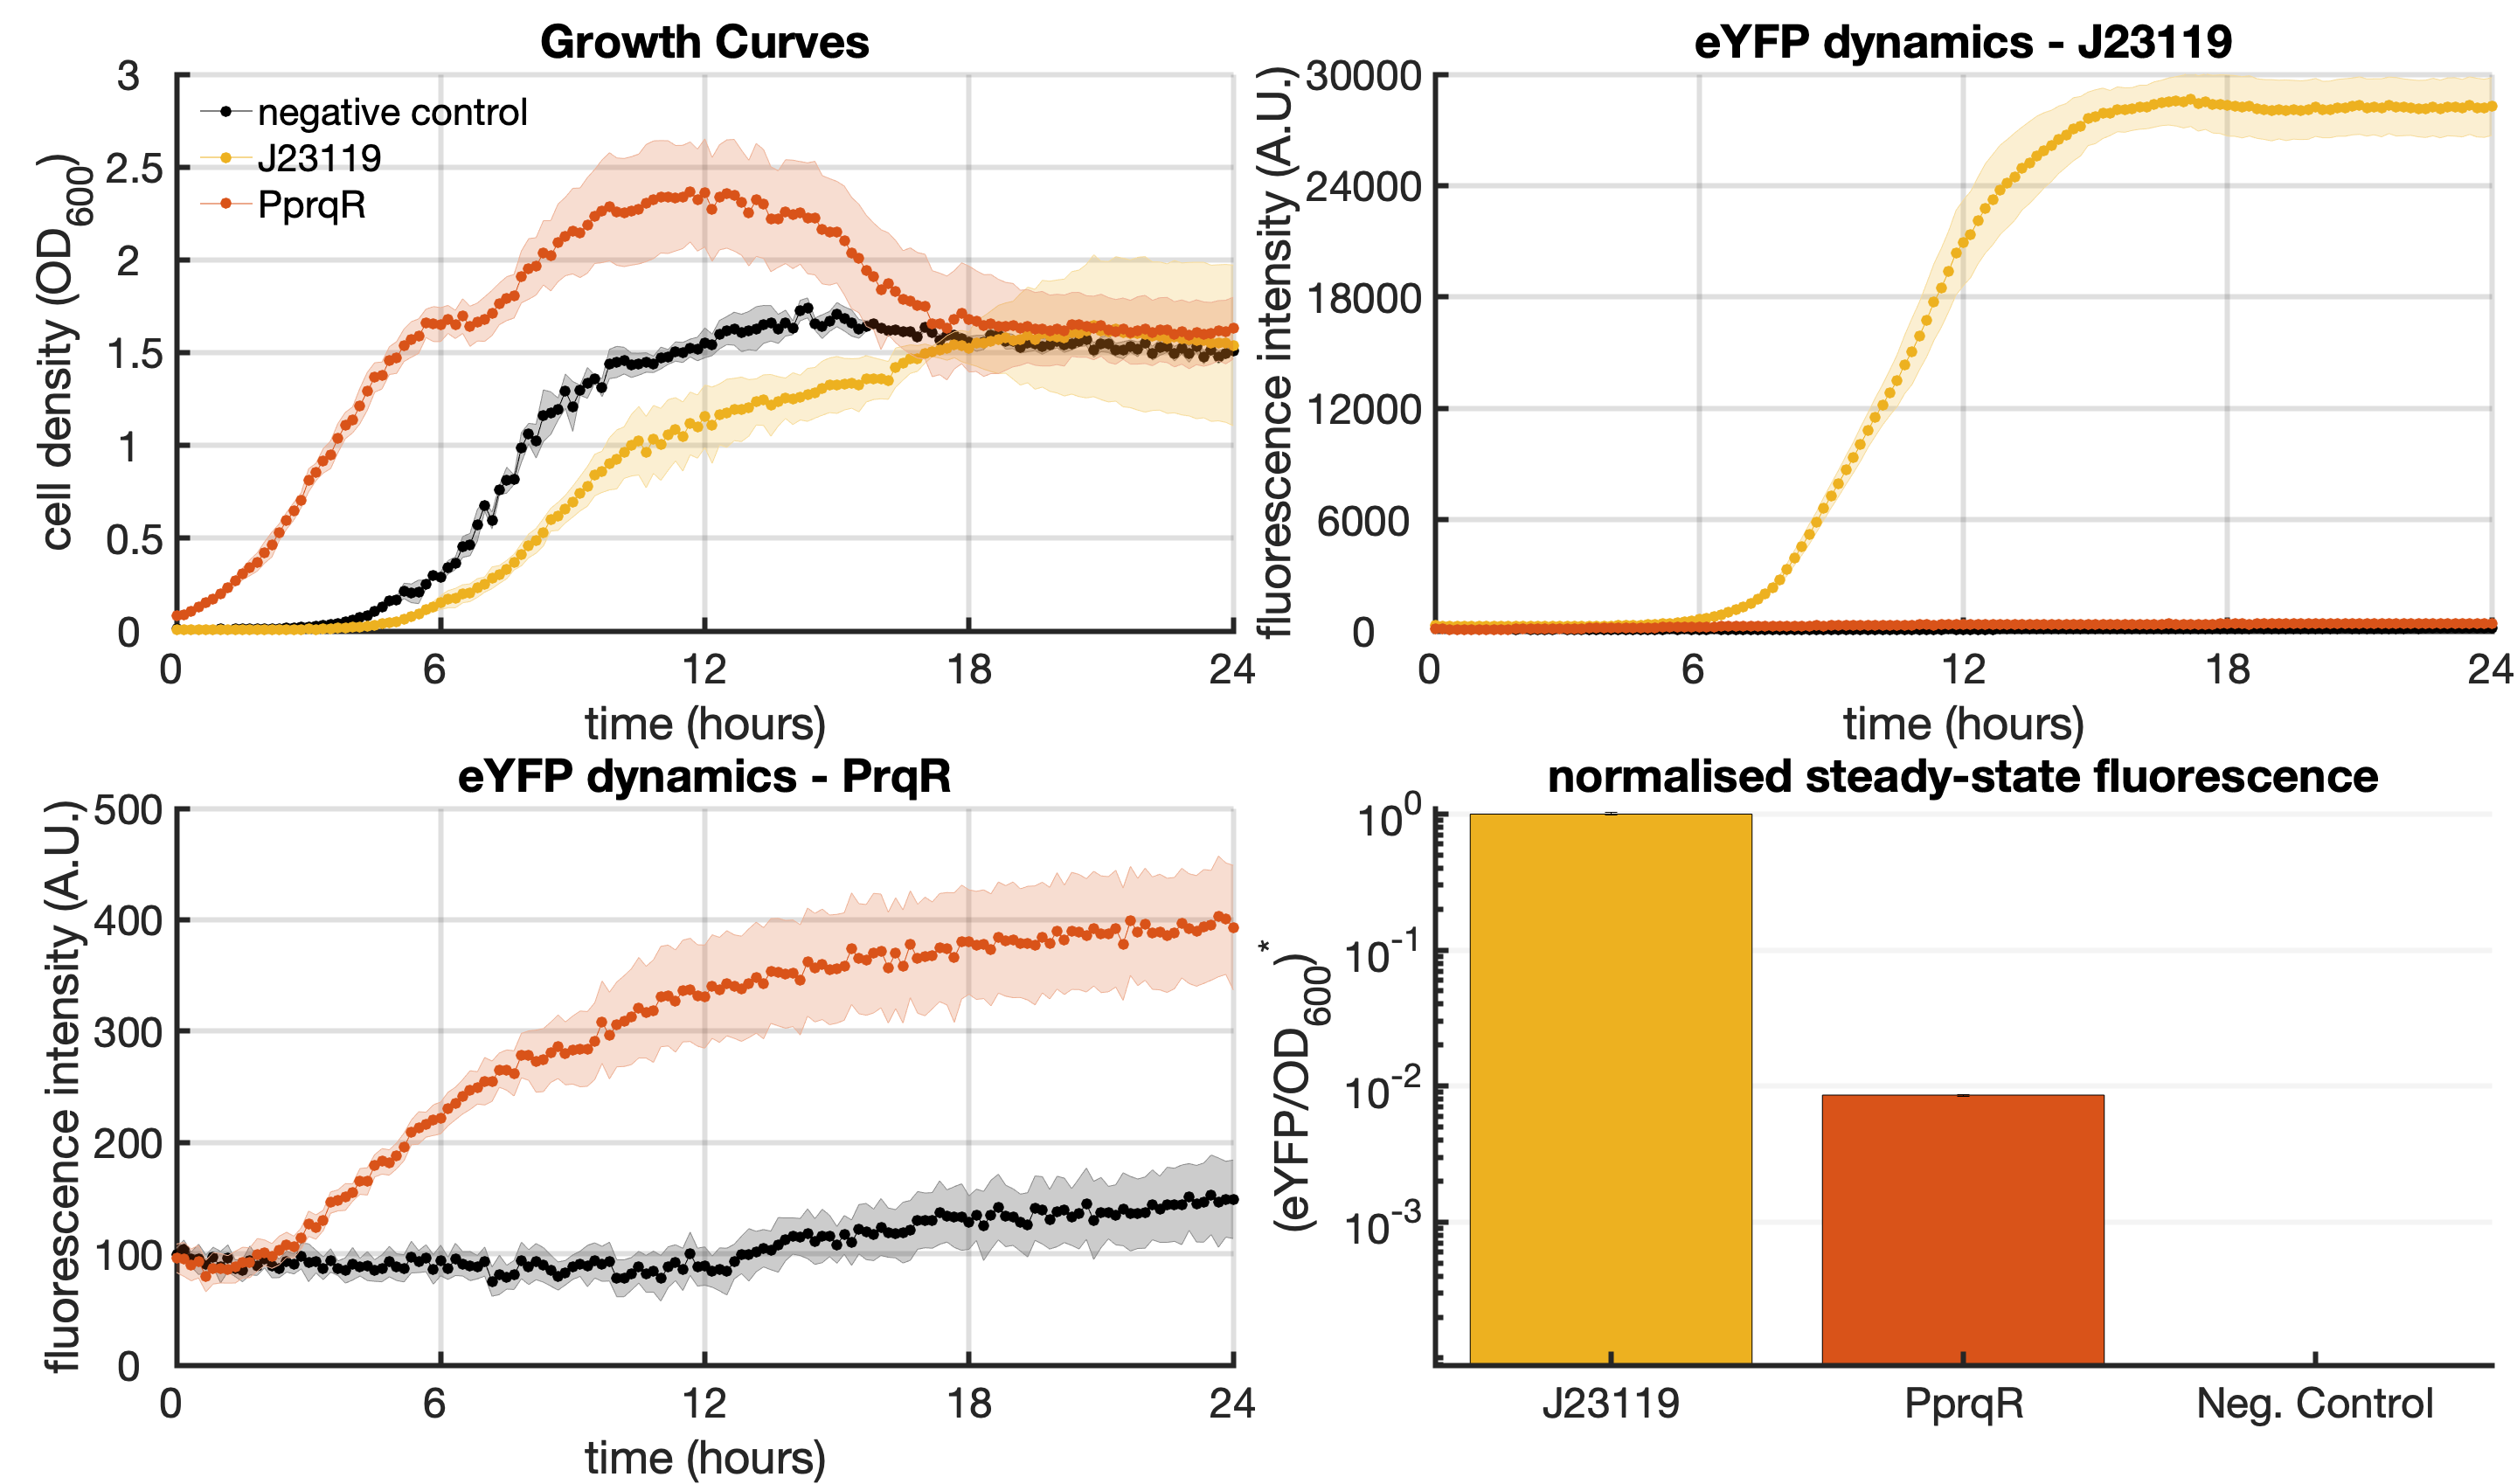
\includegraphics[width=\hsize]{figs/eYFP_J23119vsPprqR_ecoli_12_2020.png}
    \caption{Negative control: \textit{E. coli} cells transformed with the same backbone plasmid used to construct the reporter devices but no insert (no eYFP). J23119 (positive control): {E. coli} cells transformed with pAST.42, encoding eYFP under the control of the strong constitutive J23119 promoter (commonly used as reference in synthetic biology). PprqR: \textit{E. coli} cells transformed with pAST.41, encoding eYFP downstream of the PprqR promoter native to \textit{Synechocystis sp.} PCC 6803.}
    \label{fig:platereader}
\end{figure}
These results also revealed that the steady state fluorescence in cells expressing eYFP under the control of the $P_{prqR}$ promoter were two orders of magnitude lower than J23119. This is not surprising, given that  J23119 is a consensus high-strength promoter and that $P_{prqR}$ is not native to \textit{E. coli}. 


\section{Discussion and Future Work}
The material presented here is the result of the work performed since the start of the PhD project (July 2020), which has mainly focused on molecular biology to generate the genetic constructs needed to answer some of the questions posed in the introduction. 
The tables of plasmids and their DNA sequencing alignments (Tables \ref{table:level0}, \ref{table:level1}, \ref{table:levelT}) show that the modular cloning strategy developed and employed in this study was successful to assemble most of the desired genetic constructs needed for future characterisation experiments. 
The results of the transformation experiments (Section \ref{sec:trans}) also confirm that the natural transformation protocol is suitable to introduce synthetic plasmids into cyanobacterial cells. As expected, cells transformed with the the plasmids containing the spectinomycin resistance gene aadA as positive selection marker are able to grow in BG-11 plates supplemented with spectinomycin. On the other hand, no colonies appear on this same plate for the negative control condition (no plasmid added). 
Finally, the results shown in Section \ref{sec:charactreporter}, show that most of the reporter constructs (needed to quantify expression dynamics from the $P_{prqR}$ promoter) have also been successfully assembled, validated by DNA sequencing and result in the emission of a fluorescent signal in the yellow channel. The results in Figure \ref{fig:platereader} can be also used to estimate the leaky expression of the P$_{prqR}$ promoter in \textit{E. coli}. 
However, several experiments still need to be performed, and this will be the focus of future work.

In particular, the colonies that appeared after transformation of \textit{Synechocystis sp.} PCC 6803 cells with the knock-out and reporter plasmids still need to be characterised genotipically and phenotypically in order to validate the cloning strategy presented here. To do so, colonies transformed with the knock-out plasmids will be picked and PCR reactions with primers designed to amplify the genomic region supposed to be edited will be performed. By performing gel electrophoresis and DNA sequencing analyses on these amplicons, it will be possible to assess whether the CRISPR-based plasmid generated the desired deletions in the prqRA loci. For the fluorescent reporter constructs (which are plasmid-based), genotypic validation will be performed by extracting plasmid DNA from the transformed cells and sequence them with primers designed to amplify the reporter constructs. If these analyses reveal that the desired genomic modifications and reporter constructs have been introduced in \textit{Synechocystis sp.} PCC 6803, the mutants will be the subject of further characterisation experiments (e.g. growth curves) to investigate the phenotypic effects of the introduced mutations. For example, it might be possible that mutants show a significantly reduced growth, which could be due to metabolic burden caused by the synthetic genetic devices or the presence of undesired Cas12a-mediated off-target mutations . 
To overcome the burden problem, plasmids expressing the Cas12a protein under the control of weaker promoters can be employed to reduce burden (some of these plasmids have already been designed and assembled). 
To check the presence of off-target mutations, whole genome sequencing can be performed on these mutants. If these experiments will reveal high and potentially-damaging off-target activity, modifications to the design of the plasmid or the transformation protocol can be performed. For example, new plasmids can be assembled to add a counterselectable marker (e.g. sacB) in the backbone. These allow to induce the loss of the plasmid that contain such markers (and the whole CRISPR construct), to minimise the time that these plasmids are inside the cytoplasm of the cells and thus reducing the probability of off-target mutations. 

After having validated the presence of the fluorescent reporter constructs inside \textit{Synechocystis sp. PCC} 6803 cells, these genetically engineered strains will be used to quantify the dynamics of gene expression from the $P_{prqR}$ promoter when cells grow in a range of different redox conditions (e.g. in the presence of exogenous redox mediators and applied electrode potentials). By quantifying the fluorescence intensity, these experiments will reveal which conditions cause activation of the prqRA promoter and will help to understand the unknown mechanism of redox-regulation by the PrqR repressor.
Furthermore, because the PrqA protein has a predicted transporter activity, it would be interesting to quantify the exoelectrogenic activity of the $\Delta$prqR mutant. In fact - because prqR encodes the transcription factor that represses the expression of prqA - if $\Delta$prqR mutants show higher exoelectrogenic activity compared to wild-types, this would suggest that PrqA might be involved in exporting redox-mediators. This could help to understand the mechanisms of exoelectrogenesis in photosynthetic bacteria and to engineer highly exoelectrogenic strains to maximise current output in biophotovoltaics.

After having characterised the genotypes and phenotypes of the mutants, an important future experiment is to assemble and generate complementation constructs. These will be assembled by cloning the chromosomal regions that have been deleted for each knock-out mutant into replicative plasmids. These constructs will be used as controls to check if wild-type phenotypes are restored when mutants are transformed with their respective complementation plasmids. If wild-type phenotypes are not restored, this will suggest pleiotropic effects emerging from these mutations, which would be interesting to characterise.

Finally, as a result of the restrictions to laboratory access imposed by the emergence of the COVID-19 pandemic, a bioinformatic ``dry" project was devised. This aims to develop a mathematical framework to model the dynamics of gene expression of the prqRA operon in the presence of different putative redox-mediators (more in supplementary information). The theoretical predictions from this model will be useful to guide experimental design and to interpret empirical data from the characterisation of reporter plasmids.


\section*{Acknowledgements}
This research was funded by a scholarship from the Biotechnology and Biological Sciences Research Council (BBSRC-DTP). The experimental work was made possible with the supervision of Prof. Christopher Howe. The CyanoGate backbones were a kind gift from Ravi Vasudevan. The cas12a expression units were designed and gifted to me by Joshua Lawrence, to whom I am deeply grateful also for the discussions and cloning sessions we shared. I am thankful to the members of my thesis panel (Dr. Jenny Zhang, Dr. James Locke, Prof. Paul Dupree) for agreeing to be part of this project and for their helpful suggestions. Thanks also to my flatmates, Darius and Cristina, for their company and support during these unprecedented times. 

\newpage
\section*{References}
\bibliography{bibliography.bib}

\newpage

\begin{center}
\begin{LARGE}
\textbf{Supplementary Information}
\end{LARGE}\\
Alberto Scarampi (as2945@cam.ac.uk)\\
January 2021 
\end{center}

\section{Extended Methods on CyanoGate Assembly}
\label{sec:cyanogate}
All the plasmids generated in this study were assembled using Golden Gate, a DNA assembly method that employs Type-IIS restriction enzymes to cut DNA sequences at specific locations and T4 DNA ligase to paste different fragments together. Type-IIS restriction enzymes (BbsI, BsaI) cut DNA at locations outside of their hexameric recognition sequences  (e.g. GAAGAC for BBsI) and generate 4-bp long single-stranded overhangs. By designing complementary sets of overhang sequences and assigning standardised overhang to different types DNA parts (e.g. promoters, coding sequences etc...) modular cloning systems (MoClo) have been developed \citep{Weber2011}. MoClo systems are available for various synthetic biology chassis and enable a rapid and easy-to-share method to construct modular DNA libraries without proprietary tools and reagents \citep{Patron2015}.The MoClo syntax is also seen as the most suitable assembly standard for automated synthesis in DNA Foundries \citep{Chambers2016}.
For these reasons a MoClo toolbox developed for synthetic biology in cyanobacteria (CyanoGate) was used in this project. This is derived from the MoClo system for plants and microalgae (\citealt{Engler2014}; \citealt{Crozet2018}), and has been adopted by various open-source synthetic biology initiatives (\href{https://www.openplant.org/}{OpenPlant}, \href{http://parts.igem.org/Main_Page}{iGEM}) \citep{Vasudevan2019}. In order to make the DNA parts compatible with the CyanoGate toolbox,  the genes required in this project were amplified using primers containing part-specific overhangs as listed in Table \ref{table:overhangs}.

\begin{table}[H]
\begin{tabular}{|c|c|c|c|c|}
\hline
\textbf{Part Type} & \textbf{Description} & \textbf{Backbone} & \textbf{Prefix (5'-3')} & \textbf{Suffix (5'-3')} \\ \hline
Prom + 5U & promoter + RBS & pICH41295 & GGAG & AATG \\ \hline
CDS1 & coding sequence (with stop codon) & pICH41308 & AATG & GCTT \\ \hline
Cas12 gRNA & cas12a direct repeat + spacer & pICH42120 & TAGC & TTCG \\ \hline
HDR & homology directed repair template & pICH41331 & GGAG & TCGC \\ \hline
3U + Ter & 3'-UTR / terminator & pICH41276 & GCTT & CGCT \\ \hline
\end{tabular}
\caption{List of parts and overhang standards for MoClo assembly in cyanobacteria.}
\label{table:overhangs}
\end{table}

\subsection{PCR Amplification to Clone Native Genes into L0 Acceptors}
\label{sec:PCR}

The native sequences required for this project (homology repair templates, prqR, prqA) were cloned from genomic DNA extracted from \textit{Synechocystis sp.} PCC 6803. DNA was extracted from a 50 mL culture (grown to stationary phase) using the GeneJET Genomic DNA Purification Kit (Thermo Scientific)  according to the manufacturer instructions.
PCR reactions to amplify native sequence with primers containing MoClo overhangs (as listed in Table \ref{table:overhangs}) were performed using Phusion High-Fidelity Polymerase (ThermoFisher) and were carried out with the reagents listed in Table \ref{table:PCRreagents}.

\begin{table}[H]
\begin{tabular}{|c|c|c|c|}
\hline
\textbf{Component} & \textbf{[Working]} & \textbf{[Stock]} & \multicolumn{1}{l|}{\textbf{Volume to add ($\mu$l per 50 $\mu$l rxn)}} \\ \hline
Autoclaved $H_{2}O$ & 1x & 1x & up to 50 \\ \hline
Phusion HF Buffer & 1x & {\color[HTML]{333333} 5x} & 10 \\ \hline
dNTPs & 200 nM & {\color[HTML]{333333} 10000 nM} & 1 \\ \hline
Genomic DNA & {\color[HTML]{000000} 1 ng} & {\color[HTML]{333333} [nanodrop]} & 50/[nanodrop] \\ \hline
Forward Primer & 0.5 $\mu$M & 25 $\mu$M & 1 \\ \hline
Reverse Primer & 0.5 $\mu$M & 25 $\mu$M & 1 \\ \hline
Phusion$^{TM}$ Polymerase & 0.02 U/$\mu$l & 2 U/$\mu$l & 0.5 \\ \hline
\end{tabular}
\caption{List of reagents and their concentrations used for  PCR reactions}
\label{table:PCRreagents}
\end{table}

PCR reactions were carried out in 0.2 mL tubes in a PCR Thermocycler (Eppendorf). Annealing temperatures (Tm) for each set of primers were calculated with the \href{https://tmcalculator.neb.com/#!/main}{NEB Tm calculator} software using the homologous sequences as input. Cycling conditions are listed in Table \ref{table:cycling}.


\begin{table}[H]
\centering
\begin{tabular}{|l|c|c|c|}
\hline
\textbf{Cycle Step} & \multicolumn{1}{l|}{\textbf{Temp (C)}} & \multicolumn{1}{l|}{\textbf{Time  (s)}} & \multicolumn{1}{l|}{\textbf{Cycles}} \\ \hline
Initial denaturation & 98 & 30 & 1 \\ \hline
Denaturation & 98 & 5-10 sec &  \\ \cline{1-3}
Annealing & {\color[HTML]{D10E0E} \textbf{Tm}} & 10-30 sec &  \\ \cline{1-3}
Extension & 72 & 0.015 sec/bp & \multirow{-3}{*}{25-35} \\ \hline
Final Extension & 72 & 5-10 min & 1 \\ \hline
Hold & 4 & Hold & Hold \\ \hline
\end{tabular}
\caption{Parameters for thermal cycling performed to clone parts into level 0 acceptors.}
\label{table:cycling}
\end{table}

The PCR amplicons were then purified with a PCR Cleanup kit (NEB), digested and ligated in the same tube with acceptor plasmids (2:1 insert:backbone ratio), BbsI and T4 DNA Ligase. Sequences were validated by Sanger sequencing following plasmid extraction from white \textit{E. coli} colonies transformed with the assembly reactions.



\subsection{Oligo Annealing to Clone Short Parts into L0 Acceptors}
\label{sec:Annealing}

Short DNA sequences (e.g. promoters, gRNA) were constructed by annealing synthetic oligonucleotides as described by \citep{Stemmer1995}. For sequences shorter than 50 bp, double-stranded genes were assembled by designing sets of complimentary primers with desired overhangs and annealed by heating at 95$^{\circ}$C and cooling slowly to 4$^{\circ}$C. 
Longer sequences (promoters) or with secondary structures (e.g. terminators) anneal better by designing overlapping primers with 20 bp complementarity and extending them using dNTPs and a DNA polymerase enzyme (e.g. Phusion$^{TM}$) as in a PCR reaction.
\begin{figure}[H]
    \centering
    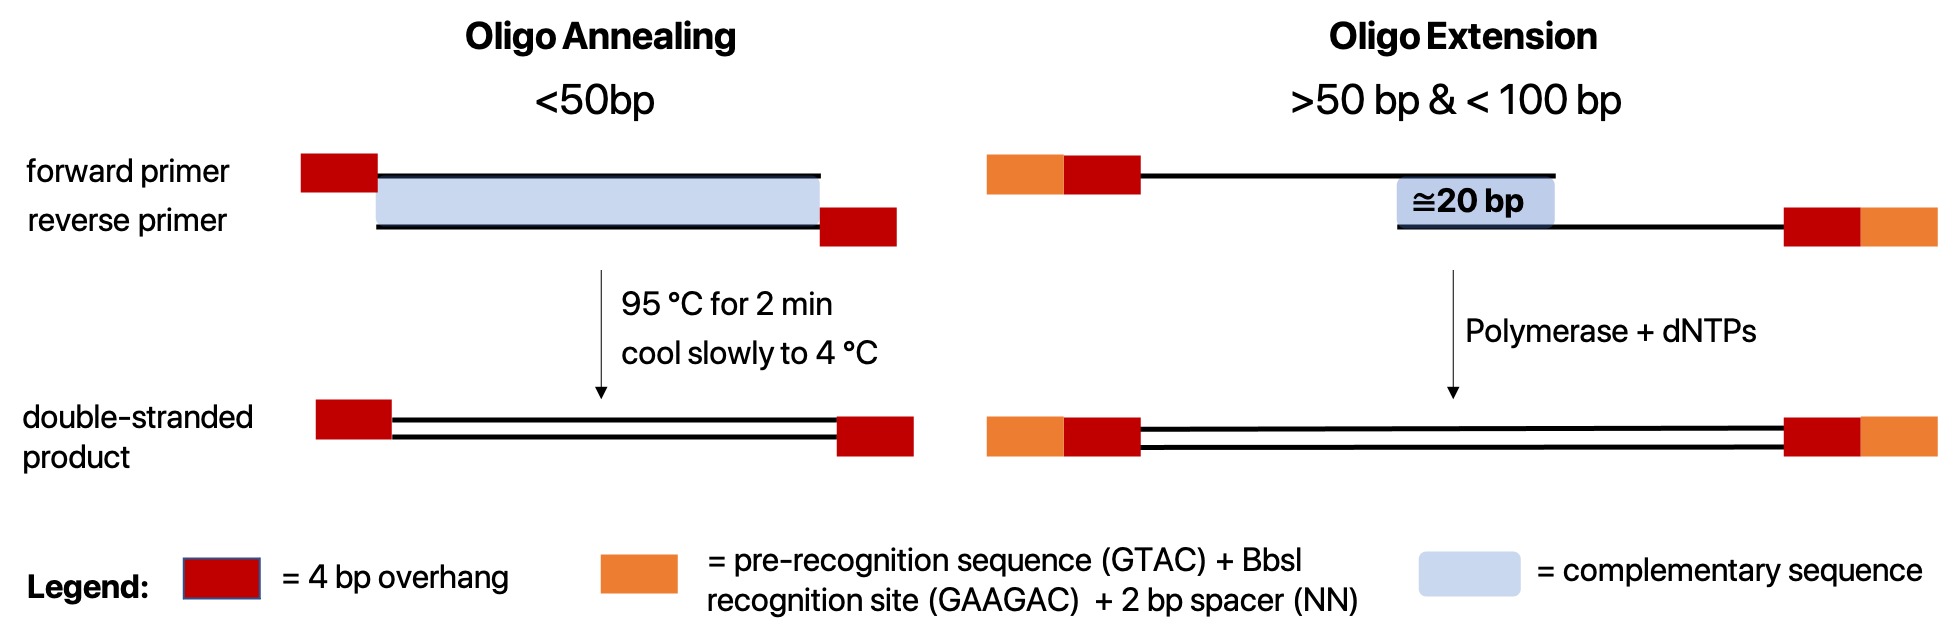
\includegraphics[width=\hsize]{figs/oligos.png}
    \caption{Strategies for annealing and extension of synthetic oligonucleotides}
\end{figure}

For annealing, complementary oligonucleotides were dissolved at a 1:1 molar ratio in an annealing buffer containing 10 mM Tris, 1 mM EDTA, 50 mM NaCl (adjusted to a pH of 8.0). Table \ref{table:annealingpar} lists the reagents and their concentrations used for these reactions.

\begin{table}[H]
\centering
\begin{tabular}{|c|c|c|c|}
\hline
\textbf{Component} & \textbf{[Working]} & \textbf{[Stock]} & \textbf{\textbf{Volume to add ($\mu$l per 50 $\mu$l rxn)}} \\ \hline
Primer F & 2.5 $\mu$M & 25 $\mu$M & 5 \\ \hline
Primer R & 2.5 $\mu$M & 25 $\mu$M & 5 \\ \hline
Annealing buffer & 1x & 10x & 5 \\ \hline
milliQ $H_{2}0$ & 1x & 1x & 35 \\ \hline
\end{tabular}
\caption{List of reagents for annealing single-stranded oligonucleotides}
\label{table:annealingpar}
\end{table}

Oligo extension was performed with the PCR parameters listed in Table \ref{table:PCRreagents} and \ref{table:cycling} with no template DNA (the primers are the template). The melting temperature was calculated using the 20 bp overlap as input in the \href{https://tmcalculator.neb.com/#!/main}{NEB Tm calculator} software.

\begin{table}[H]
\begin{adjustwidth}{-1.5cm}{-1.5cm}
\centering
\begin{tabular}{|c|c|l|c|}
\hline
{\color[HTML]{333333} \textbf{Label}} & {\color[HTML]{333333} \textbf{Primer}} & \multicolumn{1}{c|}{{\color[HTML]{333333} \textbf{DNA Sequence (5'$\rightarrow$3')}}} & {\color[HTML]{333333} \textbf{Used for:}} \\ \hline
{\color[HTML]{333333} P1} & {\color[HTML]{333333} PrqA-1F} & {\color[HTML]{333333} GTACGAAGACct\textbf{AATG}acagatatttcaatgcgatttgg} & {\color[HTML]{333333} L0 PCR} \\ \hline
{\color[HTML]{333333} P2} & {\color[HTML]{333333} PrqA-1R} & {\color[HTML]{333333} GTACGAAGACct\textbf{AAGC}ttaagatctagcaacgggaaggg} & {\color[HTML]{333333} L0 PCR} \\ \hline
{\color[HTML]{333333} P3} & {\color[HTML]{333333} PrqR-part1-1F} & {\color[HTML]{333333} GTACGAAGACct\textbf{AATG}gtttctggaaaaaggcttcgttc} & {\color[HTML]{333333} L0 PCR} \\ \hline
{\color[HTML]{333333} P4} & {\color[HTML]{333333} PrqR-part1-1R} & {\color[HTML]{333333} GTACGAAGACac\textbf{CAGG}ggagcaaaaccgtgtaag} & {\color[HTML]{333333} L0 PCR} \\ \hline
{\color[HTML]{333333} P6} & {\color[HTML]{333333} PrqR-part2-1F} & {\color[HTML]{333333} \begin{tabular}[c]{@{}l@{}}\textbf{CCTG}gaGgaccccctgcgctcccaggtcattgccactgctc\\ tgaaactggcccagctatag\end{tabular}} & {\color[HTML]{333333} annealing} \\ \hline
{\color[HTML]{333333} P7} & {\color[HTML]{333333} PrqR-part2-1R} & {\color[HTML]{333333} \begin{tabular}[c]{@{}l@{}}\textbf{AAGC}ctatagctgggccagtttcagagcagtggcaatgacctg\\ ggagcgcagggggtcttc\end{tabular}} & {\color[HTML]{333333} annealing} \\ \hline
{\color[HTML]{333333} P37} & {\color[HTML]{333333} $\Delta$PrqA-HRT-UP-3F} & {\color[HTML]{333333} GTACGAAGACTC\textbf{GGAG}tttcaatgcgatttggcatgc} & {\color[HTML]{333333} L0 PCR} \\ \hline
{\color[HTML]{333333} P38} & {\color[HTML]{333333} $\Delta$PrqA-HRT-UP-3R} & {\color[HTML]{333333} GTACGAAGACTC\textbf{TCGT}gggttatgaacaacattcccgg} & {\color[HTML]{333333} L0 PCR} \\ \hline
{\color[HTML]{333333} P45} & {\color[HTML]{333333} $\Delta$PrqA-HRT-DOWN-3F} & {\color[HTML]{333333} GTACGAAGACTC\textbf{ACGA}gtattattcatgctgaccgctggc} & {\color[HTML]{333333} L0 PCR} \\ \hline
{\color[HTML]{333333} P40} & {\color[HTML]{333333} $\Delta$PrqA-HRT-DOWN-3R} & {\color[HTML]{333333} GTACGAAGACTC\textbf{AGCG}gccaatgtatgttccgatccaaac} & {\color[HTML]{333333} L0 PCR} \\ \hline
{\color[HTML]{333333} P41} & {\color[HTML]{333333} $\Delta$PrqR-HRT-UP-2F} & {\color[HTML]{333333} GTACGAAGACTC\textbf{GGAG}tgcattatctgcggaggcg} & {\color[HTML]{333333} L0 PCR} \\ \hline
{\color[HTML]{333333} P42} & {\color[HTML]{333333} $\Delta$PrqR-HRT-UP-2R} & {\color[HTML]{333333} GTACGAAGACTC\textbf{AGCC}tccttggtgggaaag} & {\color[HTML]{333333} L0 PCR} \\ \hline
{\color[HTML]{333333} P43} & {\color[HTML]{333333} $\Delta$PrqR-HRT-DOWN-2F} & {\color[HTML]{333333} GTACGAAGACTC\textbf{GGCT}aaactggcccagctatagtttcc} & {\color[HTML]{333333} L0 PCR} \\ \hline
{\color[HTML]{333333} P44} & {\color[HTML]{333333} $\Delta$PrqR-HRT-DOWN-2R} & {\color[HTML]{333333} GTACGAAGACTC\textbf{AGCGa}aattcacgggcctctgct} & {\color[HTML]{333333} L0 PCR} \\ \hline
{\color[HTML]{333333} P10} & {\color[HTML]{333333} $\Delta$PrqRA-HRT-UP1-1F} & {\color[HTML]{333333} GTACGAAGACTC\textbf{GGAG}ctaccaacacaatgccccagagg} & {\color[HTML]{333333} L0 PCR} \\ \hline
{\color[HTML]{333333} P11} & {\color[HTML]{333333} $\Delta$PrqRA-HRT-UP1-1R} & {\color[HTML]{333333} GTACGAAGACTA\textbf{TGGC}gacctggaaataattaaaccgtccagttgg} & {\color[HTML]{333333} L0 PCR} \\ \hline
{\color[HTML]{333333} P12} & {\color[HTML]{333333} $\Delta$PrqRA-HRT-UP2-1F} & {\color[HTML]{333333} \textbf{GCCA}gtcaatttaaaaaagaatatttgcattatctgcggaggcgaaattat} & {\color[HTML]{333333} annealing} \\ \hline
{\color[HTML]{333333} P13} & {\color[HTML]{333333} $\Delta$PrqRA-HRT-UP2-1R} & {\color[HTML]{333333} \begin{tabular}[c]{@{}l@{}}\textbf{AGTC}ATAATTTCGCCTCCGCAGATAATGcaaatat\\ tcttttttaaattgac\end{tabular}} & {\color[HTML]{333333} annealing} \\ \hline
{\color[HTML]{333333} P18} & {\color[HTML]{333333} $\Delta$PrqRA-HRT-DOWN-1F} & {\color[HTML]{333333} GTACGAAGACga\textbf{GACT}cccgttgctagatcttaatccataattgcc} & {\color[HTML]{333333} L0 PCR} \\ \hline
{\color[HTML]{333333} P19} & {\color[HTML]{333333} $\Delta$PrqRA-HRT-DOWN-1F} & {\color[HTML]{333333} GTACGAAGACgc\textbf{AGCG}agggaggagcgttaaagggaac} & {\color[HTML]{333333} L0 PCR} \\ \hline
{\color[HTML]{333333} P54} & {\color[HTML]{333333} PmScarletI-1F} & {\color[HTML]{333333} GTACGAAGACct\textbf{AATG}agtaaaggagaagctgtg} & {\color[HTML]{333333} L0 PCR} \\ \hline
{\color[HTML]{333333} P55} & {\color[HTML]{333333} PmScarletI-1R} & {\color[HTML]{333333} GTACGAAGACct\textbf{AAGC}ttatttgtatagttcatccatgcc} & {\color[HTML]{333333} L0 PCR} \\ \hline
{\color[HTML]{333333} P20} & {\color[HTML]{333333} Cas12a-gRNA-prqR-1F} & {\color[HTML]{333333} \begin{tabular}[c]{@{}l@{}}\textbf{TAGC}TAATTTCTACTAAGTGTAGATtggaaa\\ cattgcatcaggaactt\end{tabular}} & {\color[HTML]{333333} annealing} \\ \hline
{\color[HTML]{333333} P21} & {\color[HTML]{333333} Cas12a-gRNA-prqR-1R} & {\color[HTML]{333333} \begin{tabular}[c]{@{}l@{}}\textbf{AAGC}aagttcctgatgcaatgtttccaATCTACACTT\\ AGTAGAAATTA\end{tabular}} & {\color[HTML]{333333} annealing} \\ \hline
{\color[HTML]{333333} P22} & {\color[HTML]{333333} Cas12a-gRNA-prqA-1F} & {\color[HTML]{333333} \begin{tabular}[c]{@{}l@{}}\textbf{TAGC}TAATTTCTACTAAGTGTAGATagattccta\\ tttgaatgtgatgg\end{tabular}} & {\color[HTML]{333333} annealing} \\ \hline
{\color[HTML]{333333} P23} & {\color[HTML]{333333} Cas12a-gRNA-prqA-1R} & {\color[HTML]{333333} \begin{tabular}[c]{@{}l@{}}\textbf{AAGC}ccatcacattcaaataggaatctATCTACACTTA\\ GTAGAAATTA\end{tabular}} & {\color[HTML]{333333} annealing} \\ \hline
{\color[HTML]{333333} P58} & {\color[HTML]{333333} PprqR-3F} & {\color[HTML]{333333} \begin{tabular}[c]{@{}l@{}}GTACGAAGACCT\textbf{GGAG}gtatcttgaaagtgtccaac\\ caactggacggtttaattatttccaggtcGCc\end{tabular}} & {\color[HTML]{333333} extension} \\ \hline
{\color[HTML]{333333} P59} & {\color[HTML]{333333} PprqR-3R} & {\color[HTML]{333333} \begin{tabular}[c]{@{}l@{}}GTACGAAGACCT\textbf{CATT}ataatttcgcctccgcagata\\ atgcaaatattcttttttaaattgacagGCgacctggaaataattaaaccgtcc\end{tabular}} & {\color[HTML]{333333} extension} \\ \hline
{\color[HTML]{333333} P60} & {\color[HTML]{333333} PprqA-2F} & {\color[HTML]{333333} GTACGAAGACCT\textbf{GGAG}catatttaataactattttagttctttgg} & {\color[HTML]{333333} extension} \\ \hline
{\color[HTML]{333333} P61} & {\color[HTML]{333333} PprqA-2R} & {\color[HTML]{333333} GTACGAAGACCT\textbf{CATT}agcattgacccaaagaactaaaatagttat} & {\color[HTML]{333333} extension} \\ \hline
{\color[HTML]{333333} P62} & {\color[HTML]{333333} TprqR-2F} & {\color[HTML]{333333} \begin{tabular}[c]{@{}l@{}}GTACGAAGACCT\textbf{GCTT}tttcccaatttttcatcttttgc\\ cgacgtttgccaaatggtttccagcgctggttggtggctctaggg\end{tabular}} & {\color[HTML]{333333} extension} \\ \hline
{\color[HTML]{333333} P63} & {\color[HTML]{333333} TprqR-2R} & {\color[HTML]{333333} \begin{tabular}[c]{@{}l@{}}GTACGAAGACCT\textbf{AGCG}aaaaaacaaattttctctaa\\ agatattccctagagccaccaaccagcg\end{tabular}} & {\color[HTML]{333333} extension} \\ \hline
\end{tabular}
\end{adjustwidth}
\captionsetup{width= 7.7in}
\caption{List of oligonucleotide sequences used during this project. Uppercase letters denote overhang sequences (4bp restriction overhangs in bold), lowercase correspond to sequences homologous to genomic loci.}
\label{table:primers}
\end{table}

\subsection{Modular Assembly of CRISPR Knock-Out Plasmids}
The native or synthetic DNA parts assembled as above were used to assemble knock-out plasmids required to generate the $\Delta$prqR, $\Delta$prqA, $\Delta$prqRA mutants. Figure \ref{fig:KOstrategy} illustrates the Golden Gate cloning strategy employed to assemble the level 0 parts into level T knock-out plasmids. 


\begin{figure}[H]
    \centering
    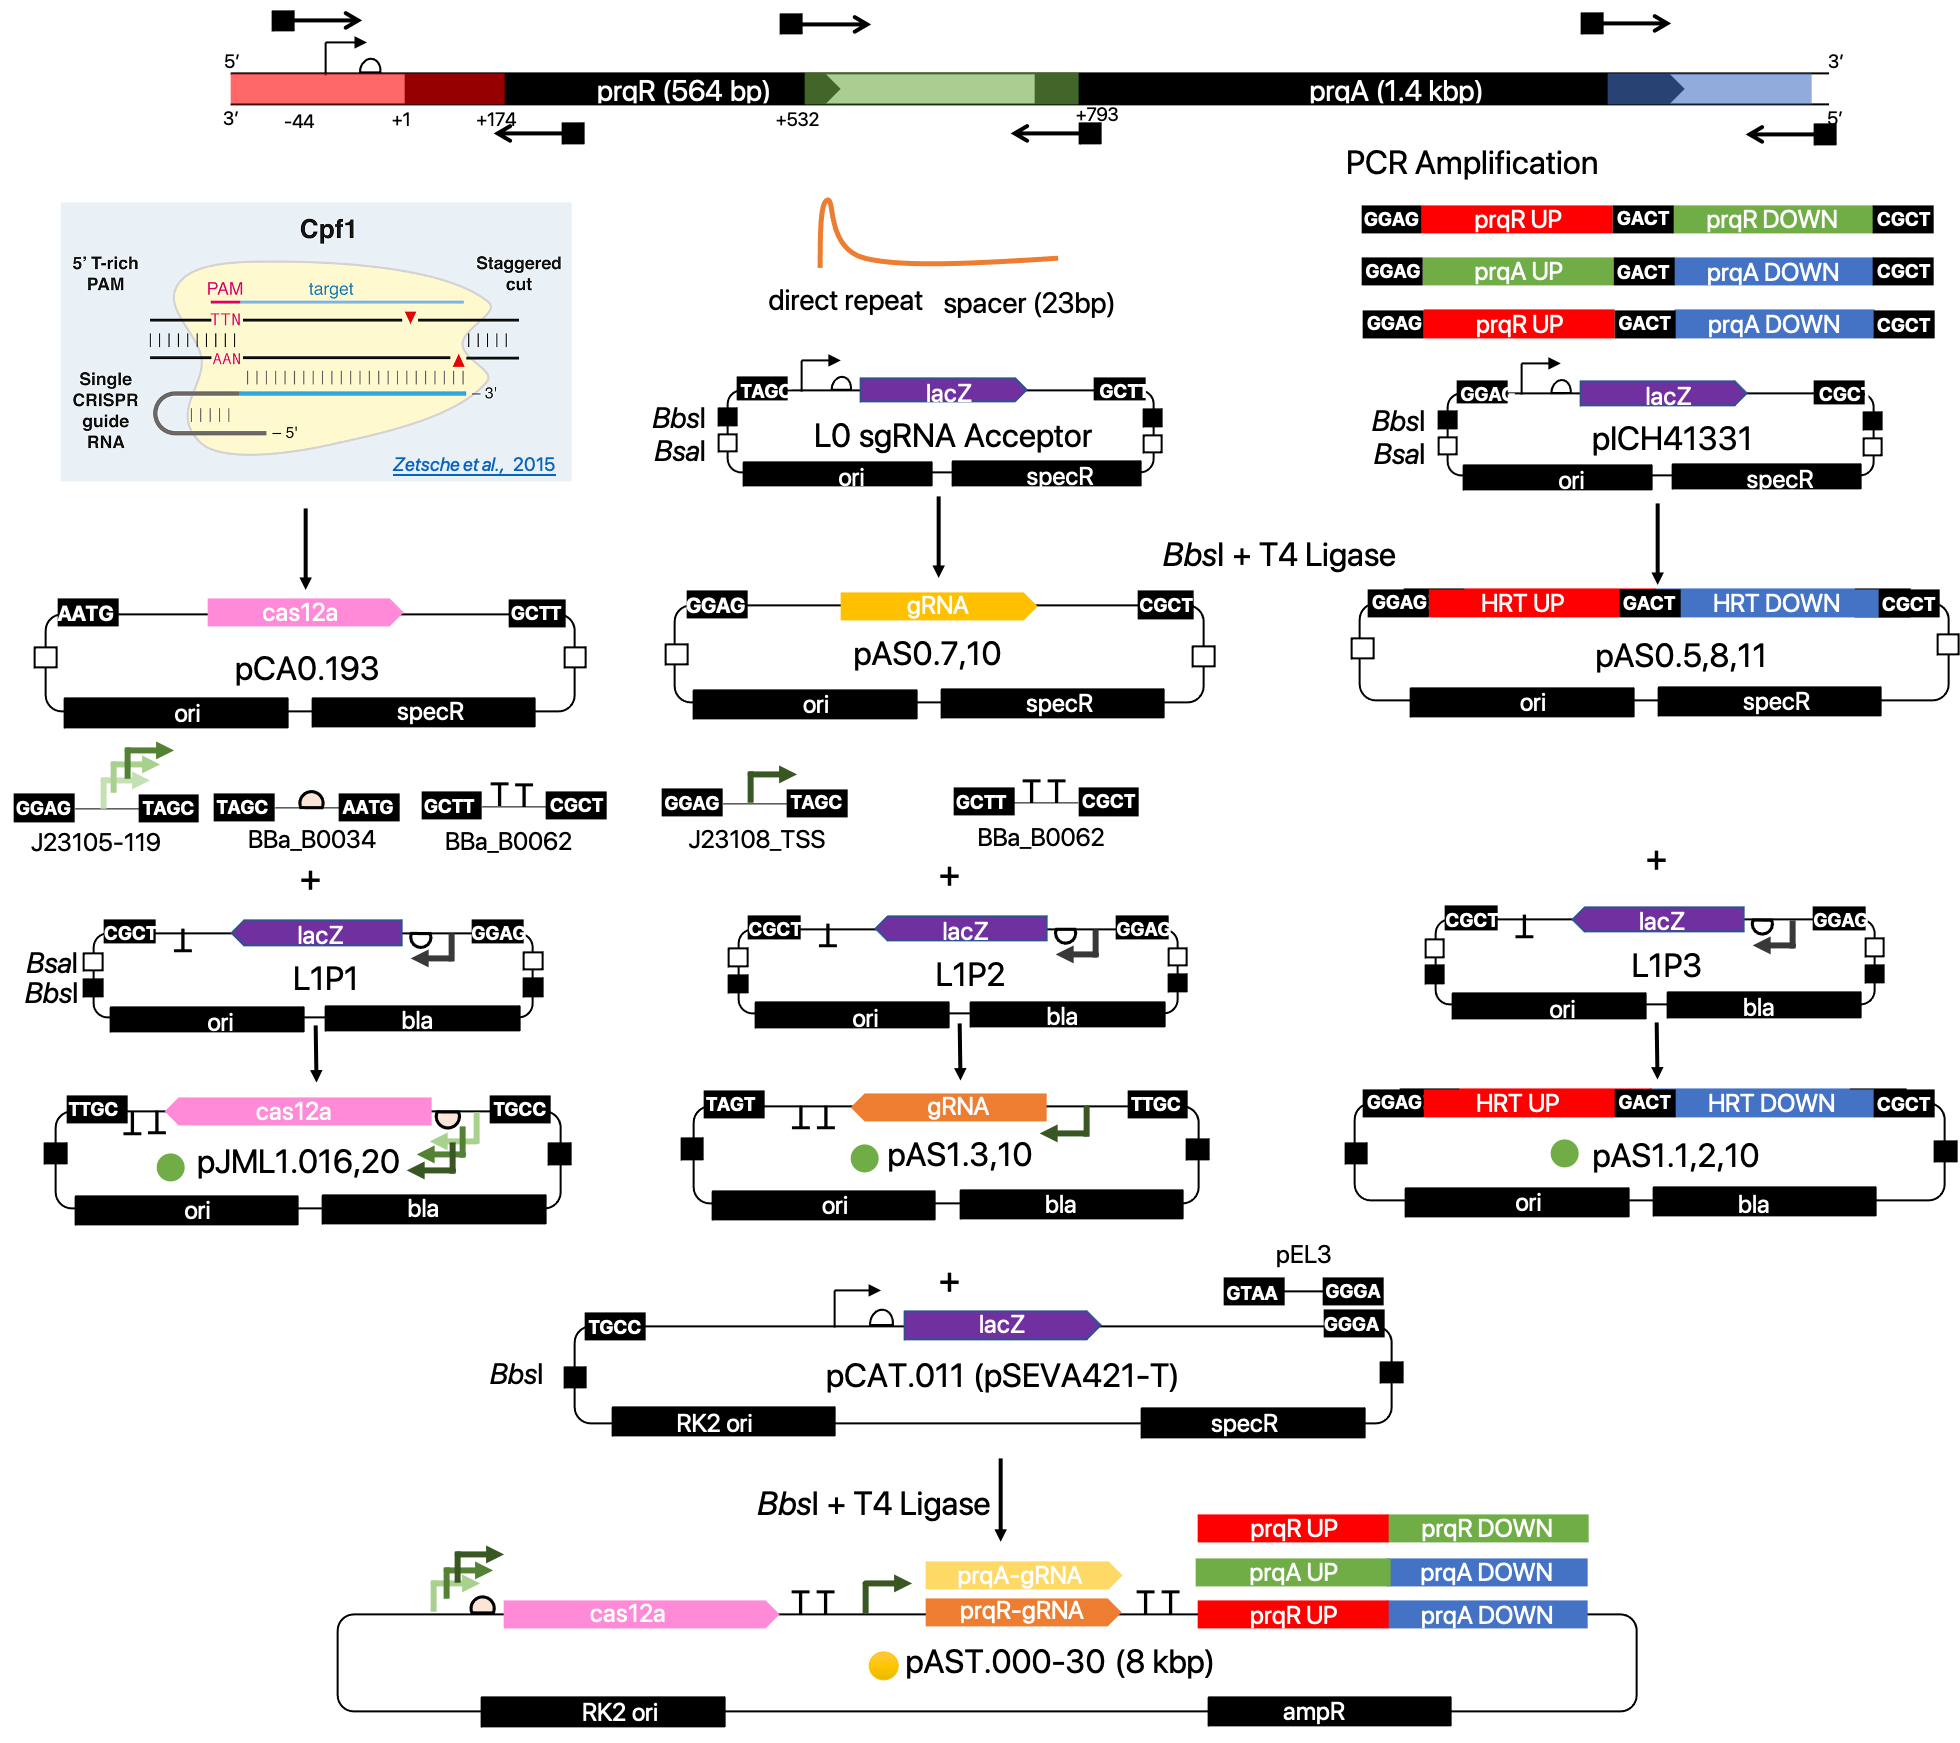
\includegraphics[width=\hsize]{figs/ASgate.png}
    \caption{Outline of the cloning strategy to construct modular knock-out plasmids. White and black squares indicate BbsI and BsaI recognition sites respectively. specR: spectinomycin resistance; bla: ampicillin/carbenicillin resistance; lacZ: beta-galactosidase coding sequence used for blue-white screening upon induction with IPTG and X-Gal.}
    \label{fig:KOstrategy}
\end{figure}

\newpage

\subsection{Level 0 Assembly}
To clone PCR products into MoClo acceptors. Restriction: BbsI; selection: spectinomycin.

\subsubsection{Homology Repair Templates}

\begin{figure}[H]
    \centering
    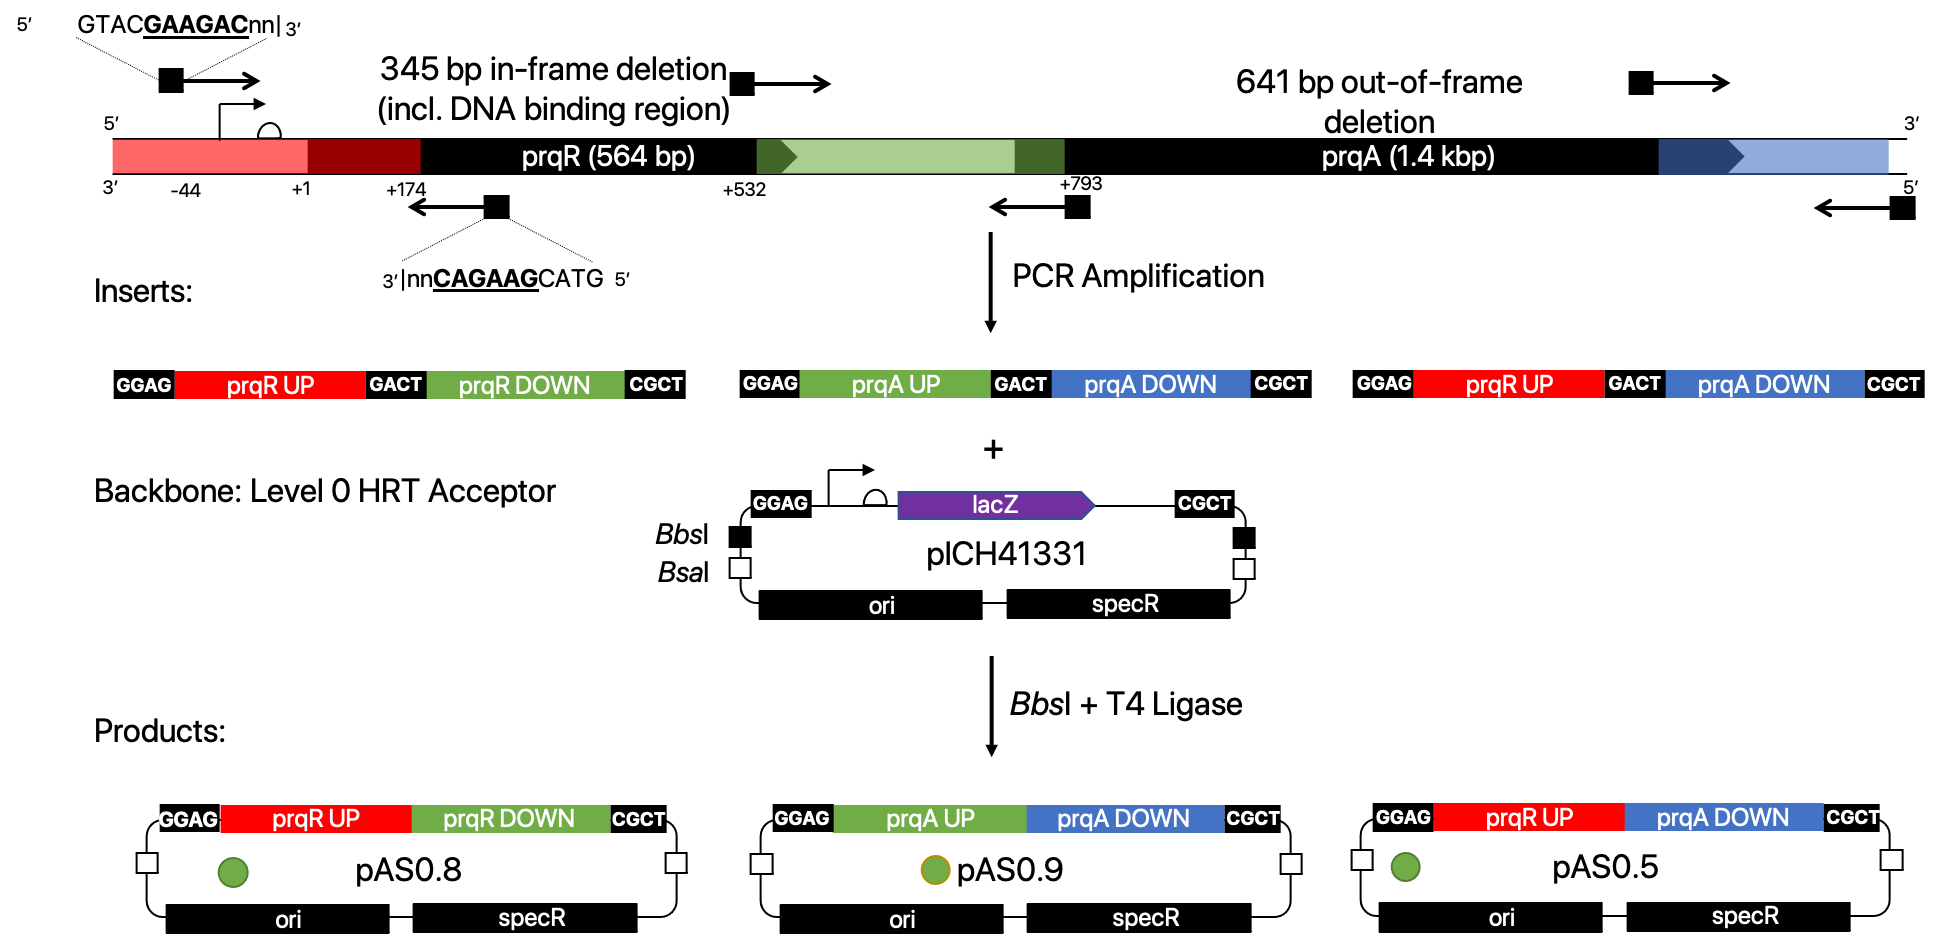
\includegraphics[width=\hsize]{figs/HRT.png}
    \caption{Cloning Homology Repair Templates into Level 0 Acceptors}
\end{figure}

\subsubsection{Coding Sequences}

\begin{figure}[H]
    \centering
    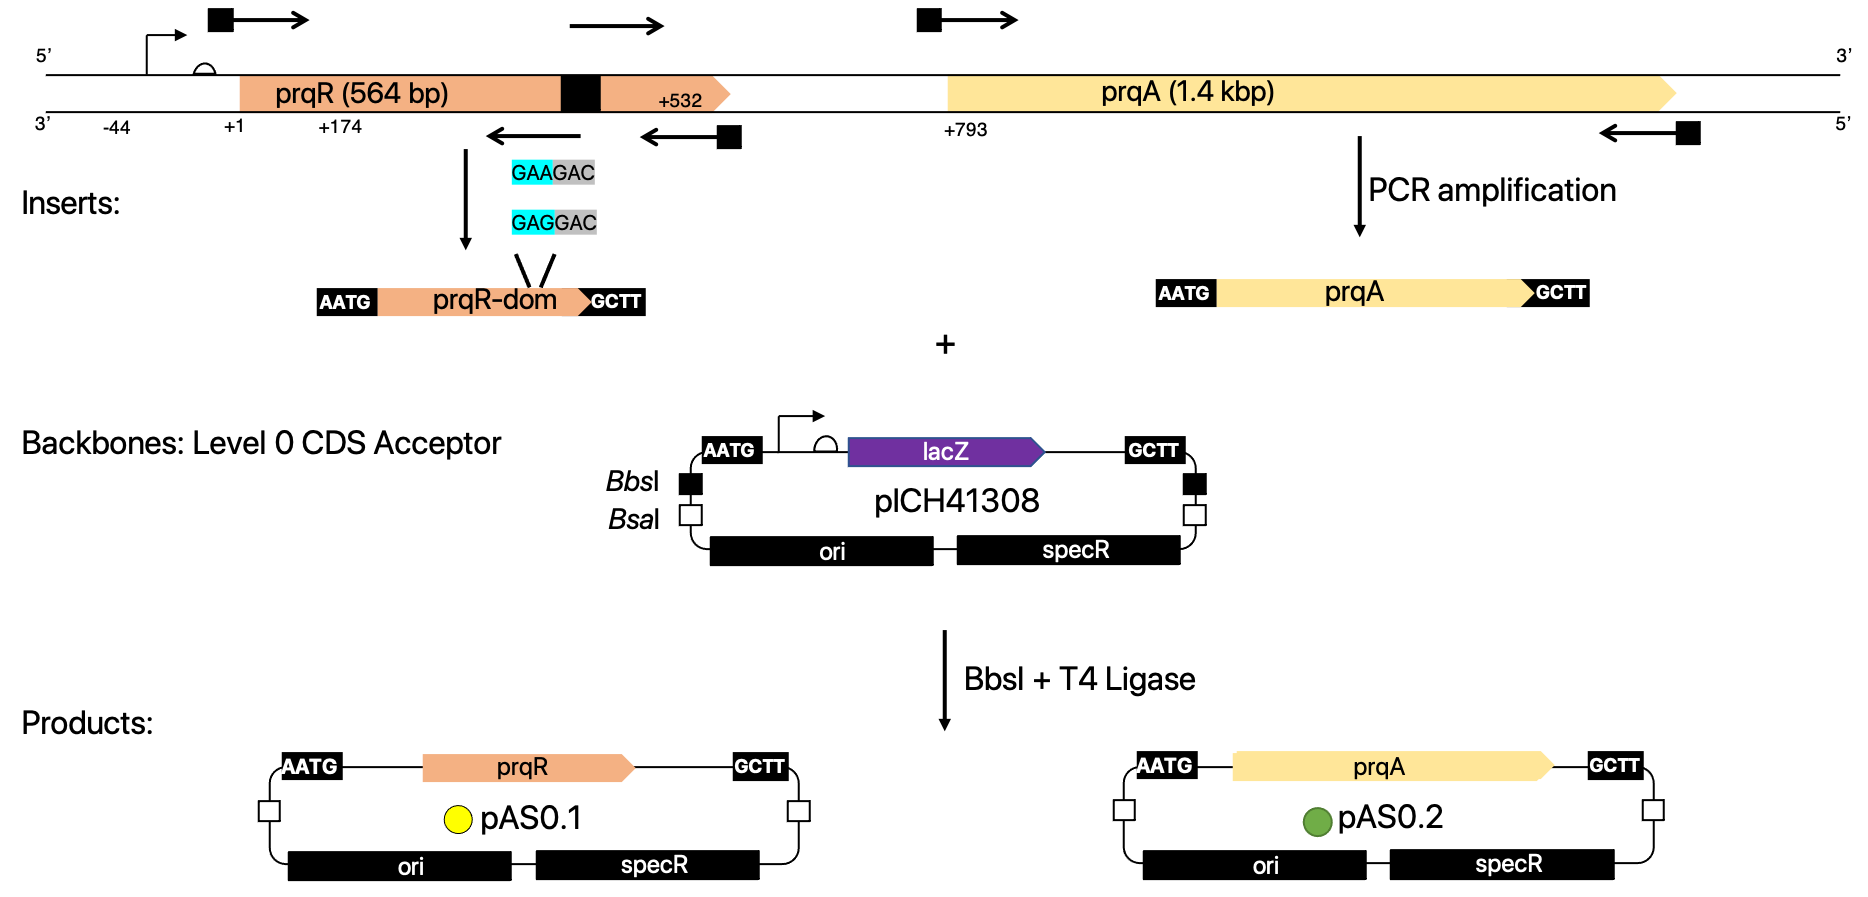
\includegraphics[width=\hsize]{figs/CDS.png}
    \caption{Cloning Coding Sequences into Level 0 Acceptors}
\end{figure}

\subsubsection{Cas12a gRNAs}

\begin{figure}[H]
    \centering
    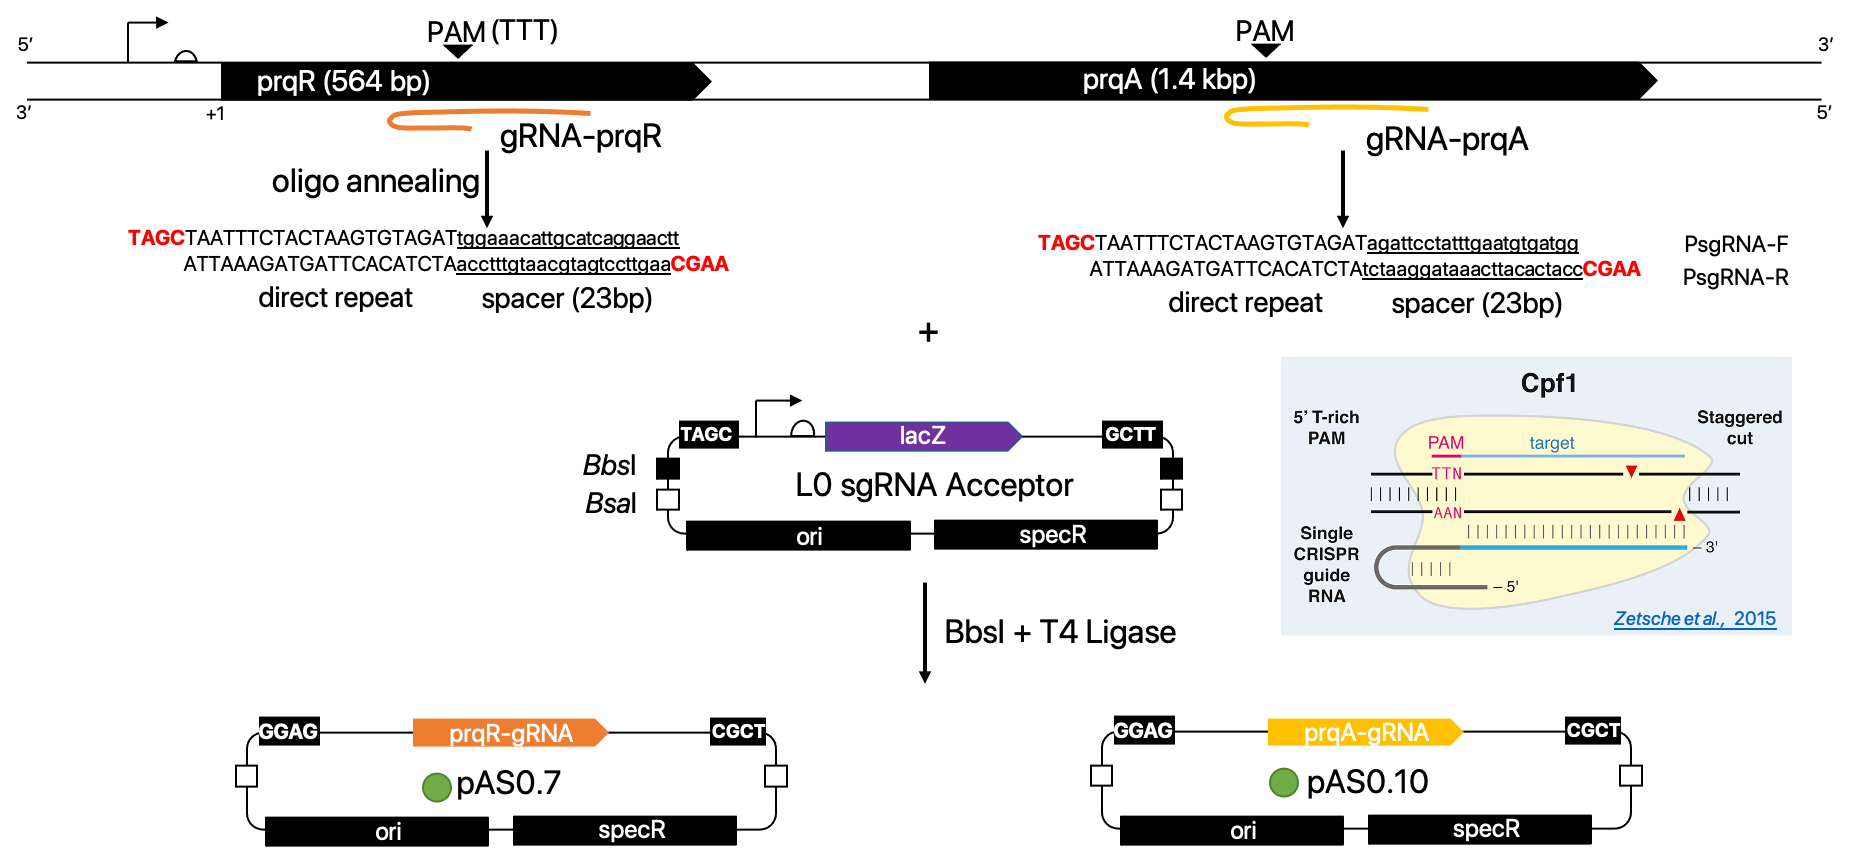
\includegraphics[width=\hsize]{figs/gRNA.png}
    \caption{Cloning Cas12a gRNA via oligo annealing into Level 0  acceptors}
\end{figure}
All the level 0 plasmids marked with a green dot has been validated by DNA sequencing. The coding sequence for the PrqR repressor contains a BbsI recognition site and still needs to be domesticated. Figure \ref{fig:L0} illustrates the library of DNA parts constructed during this project.
\begin{figure}[H]
    \centering
    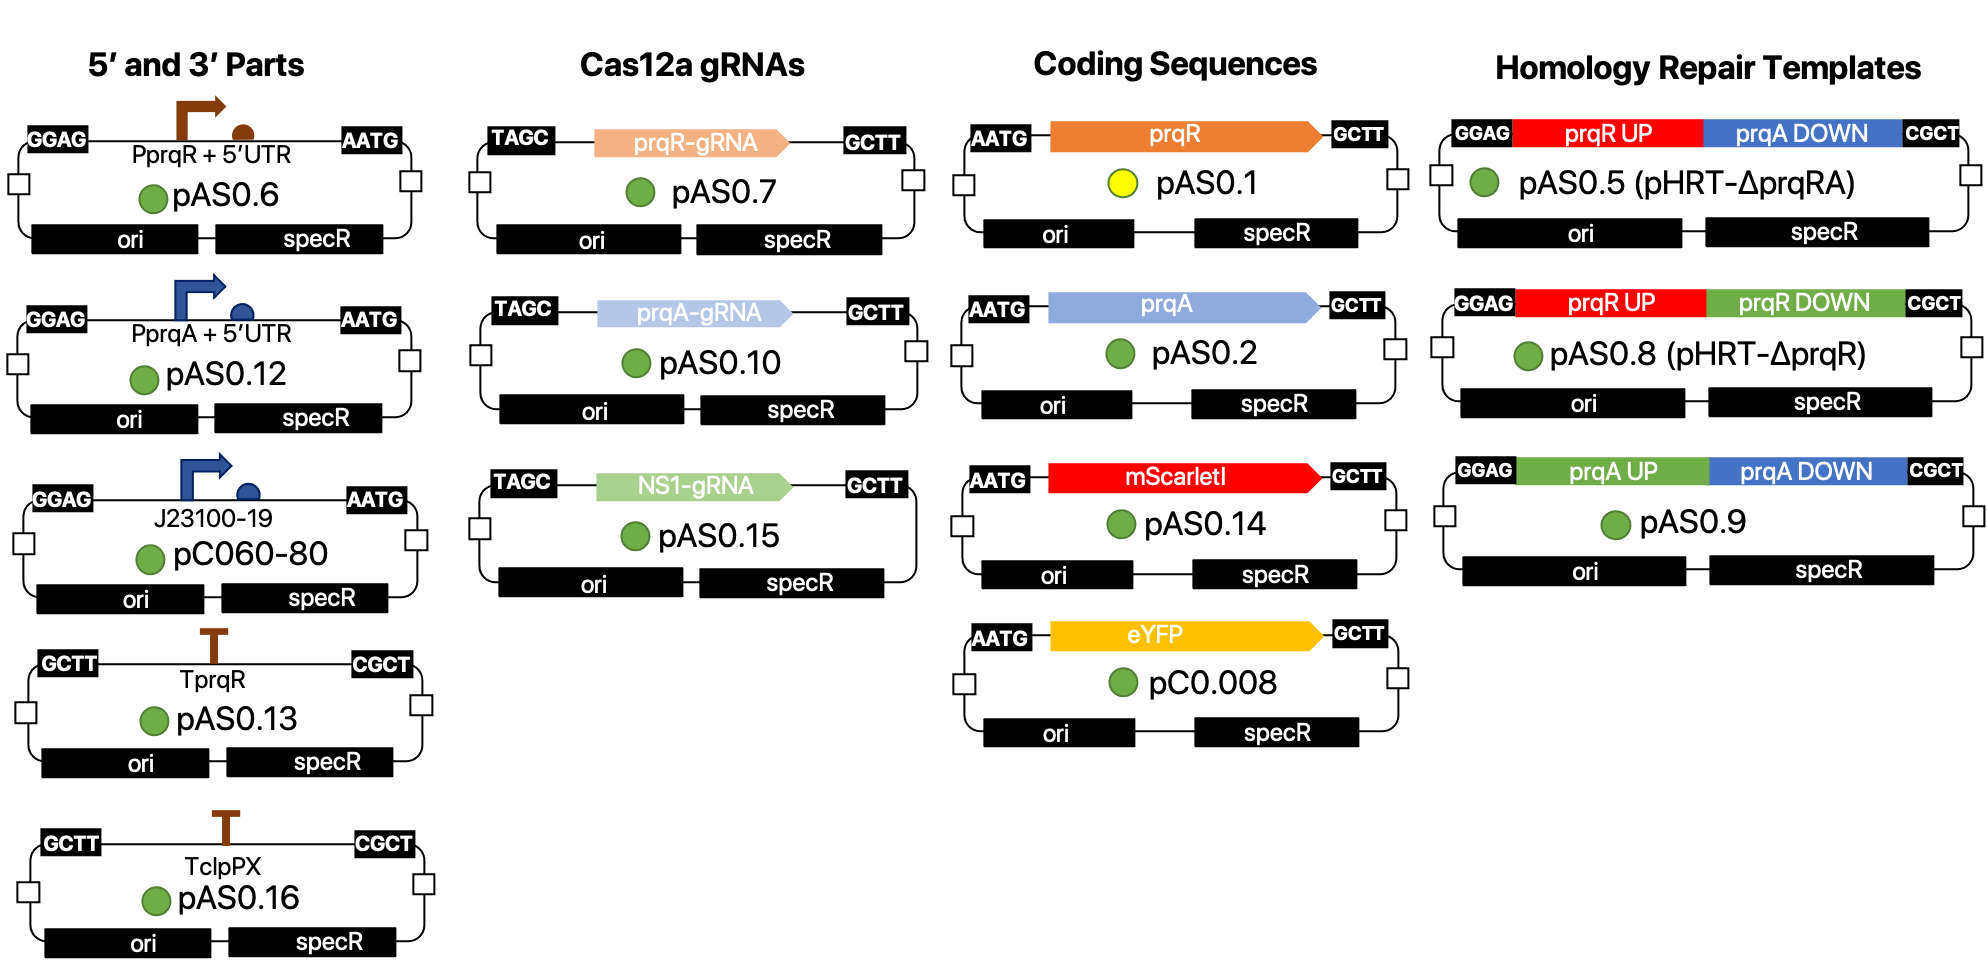
\includegraphics[width=\hsize]{figs/l0.png}
    \caption{Summary of level 0 library of plasmids assembled until now. Green dots indicate DNA parts validated by DNA sequencing. The pAS0.1 plasmid (yellow circle) contains an undesired mutation that still needs to be domesticated.}
    \label{fig:L0}
\end{figure}

\subsubsection{Level 1 Assembly}
Level 1 assembly reactions consist in cloning the inserts contained in level 0 plasmids into level 1 acceptor backbones. During this assembly reaction, the orientation of the level 0 parts will be inversed (genes will be in the reverse strand). This is not a problem as they will be reinverted in the next level T assembly reactions.
The CyanoGate level 1 acceptors are derived from the PlantGate MoClo toolbox. There are up to 7 different level 1 acceptors (L1P1, L1P2, ..., L1P7), which specify the position of level 1 expression units for multigene assembly into the final level T plasmids. For example, if the final plasmid requires two expression cassettes, one upstream of the other, the first unit will need to be cloned in L1P1, whilst the second one in L1P2. After level T assembly, the two cassettes will be found one after the other (separated by a 4 bp scar), in the forward strand in the level T plasmid. 


\begin{figure}[H]
    \centering
    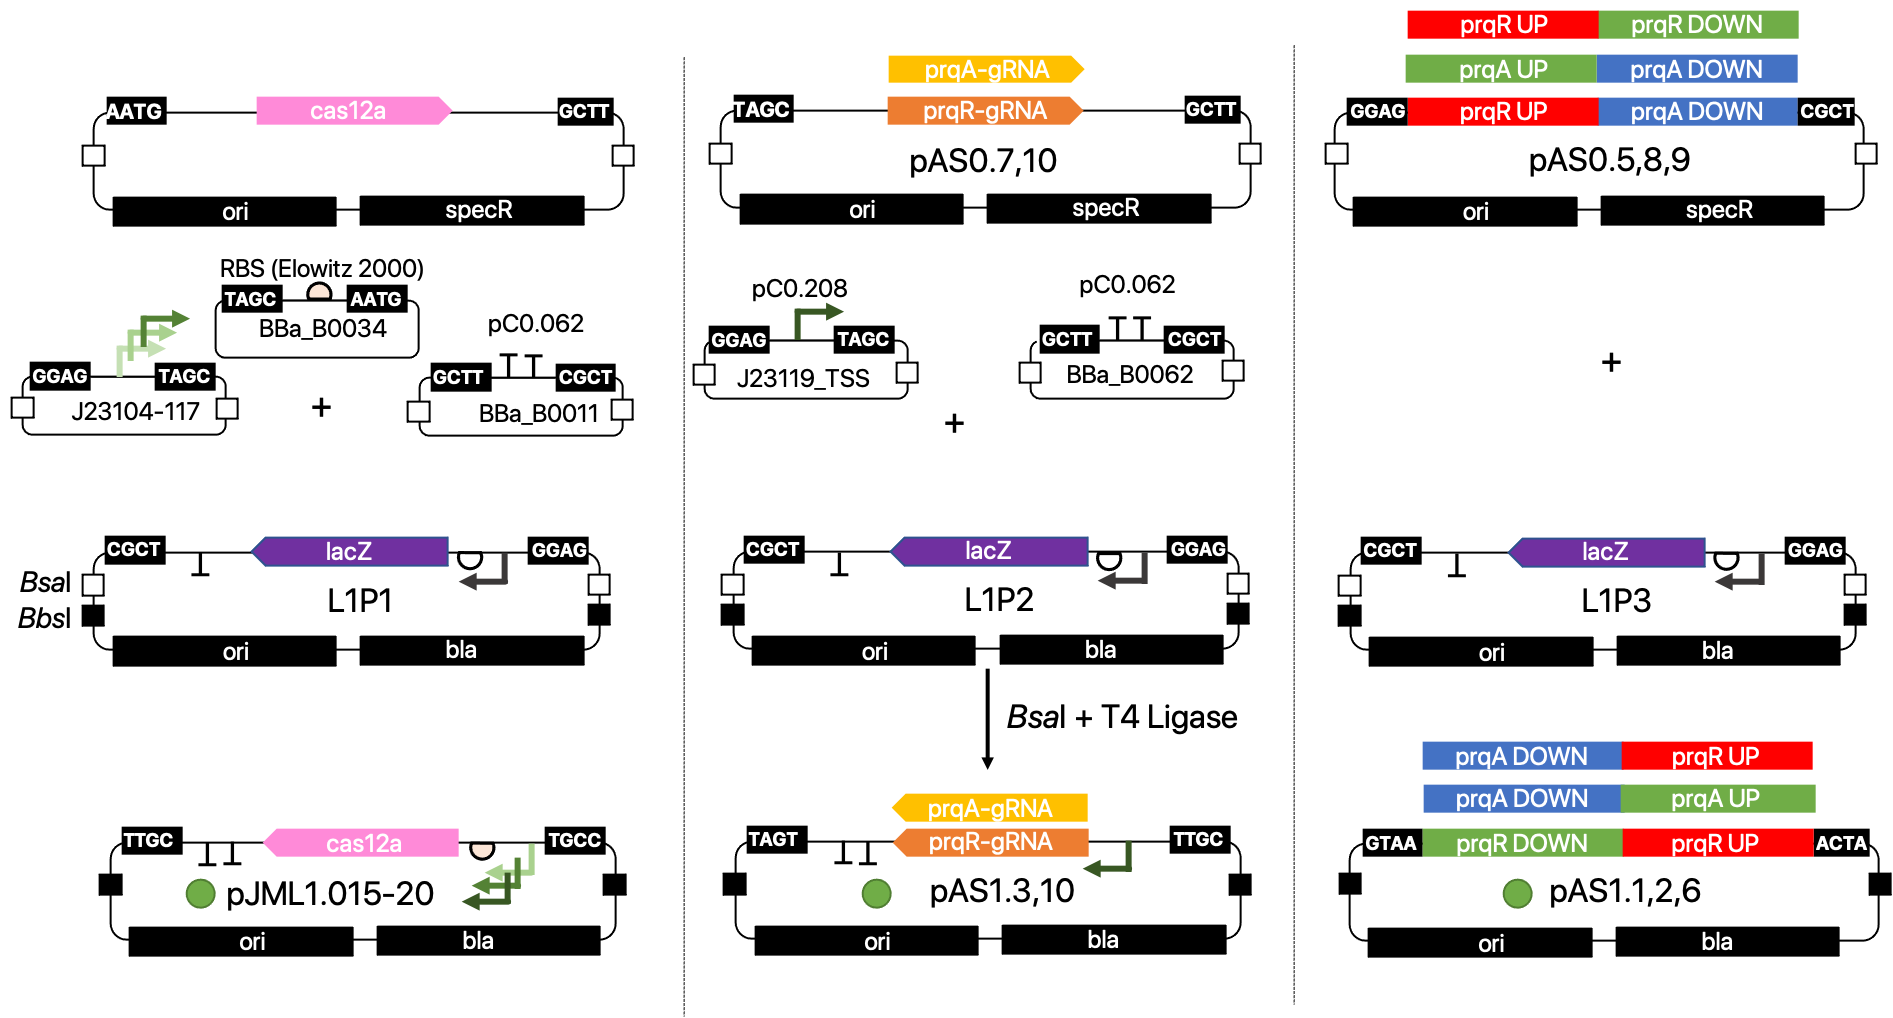
\includegraphics[width=\hsize]{figs/l1.png}
    \caption{Overview of the level 1 plasmids designed and assembled in this project.}
\end{figure}

\subsubsection{Level T Assembly}
Level T assembly consists in cloning multigene constructs from level 1 expression cassettes into level T acceptor backbones. Level T acceptors are shuttle vectors that replicate both in \textit{E. coli} and in a range of cyanobacteria hosts. This assembly step is performed with BbsI for restriction digestion. Selection depends on the antibiotic resistance gene encoded in the level T backbone. For the pCAT.011 (pSEVA421-T) backbone plasmid used in this study, spectinomycin was used as positive selection.
This plasmid is a MoClo-compatible vector derived from pSEVA421 and carries the RK2 replicative origin and has an average copy number of $\approx$ 10 in \textit{Synechocystis} \citep{Vasudevan2019}.

\subsubsection{Cloning level 1 parts into level T acceptors}
\begin{figure}[H]
    \centering
    \includegraphics[width=\hsize]{figs/LT.png}
    \caption{Cloning Level 1 into Level T Acceptors. SPT are sequencing primers designed to span the entire insert sequence for Sanger DNA sequencing.}
\end{figure}


\begin{figure}[H]
    \centering
    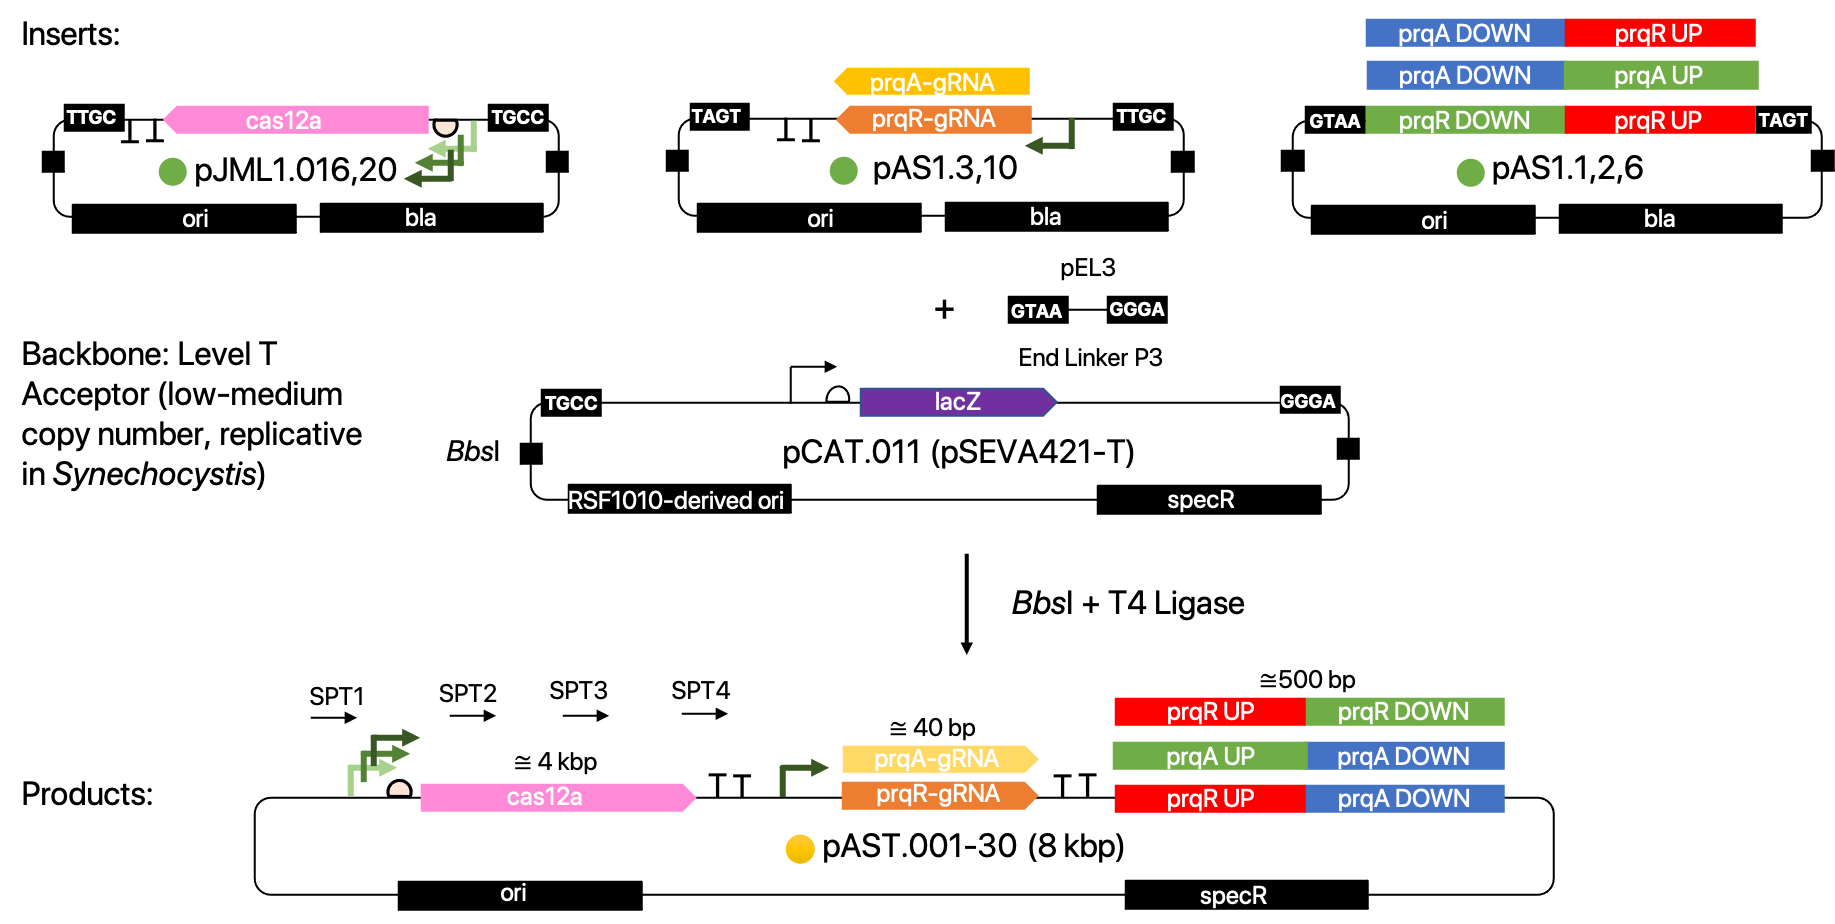
\includegraphics[width=\hsize]{figs/lt.png}
    \caption{Overview of level T plasmids designed and assembled in this project}
\end{figure}

\section{Construction of Fluorescent Reporter Plasmids}
In order to quantify the expression dynamics from native genes, a common approach in synthetic biology is to construct synthetic gene circuits by rewiring the  transcription factors and promoters to create novel regulatory topologies \citep{Chen2018}. During this project, the native PrqR transcription factor and the P$_{prqR}$ promoter have been used to construct synthetic gene circuits containing fluorescent reporter proteins regulated by these regulatory sequence.
To do so, the P$_{prqR}$ promoter sequence had to be annotated in the genome of \textit{Synechocystis sp.} PCC 6803. This was performed by identifying the DNA sequence extending 100 bp upstream of the first A nucleotide in the start codon (ATG) of the prqR gene. As shown in Fig. \ref{fig:promoteranal}, this sequence was aligned for comparison with the J23119 promoter sequence (which is a consensus eubacterial promoter commonly used as reference in synthetic biology). Using promoter and RBS prediction softwares (\href{http://www.bacpp.bioinfoucs.com/home}{BacPP}, \href{https://salislab.net/software/}{RBS calculator}), it was possible to identify certain features in the promoter sequence, such as the ribosome binding sites (RBS in green), the -10 and -35 regions (in yellow and purple, the sequences bound by the RNA polymerase sigma factors). The operator sequences (regions bound by repressor PrqR) were previously annotated by \citep{Babykin2003}.

\begin{figure}[H]
    \centering
    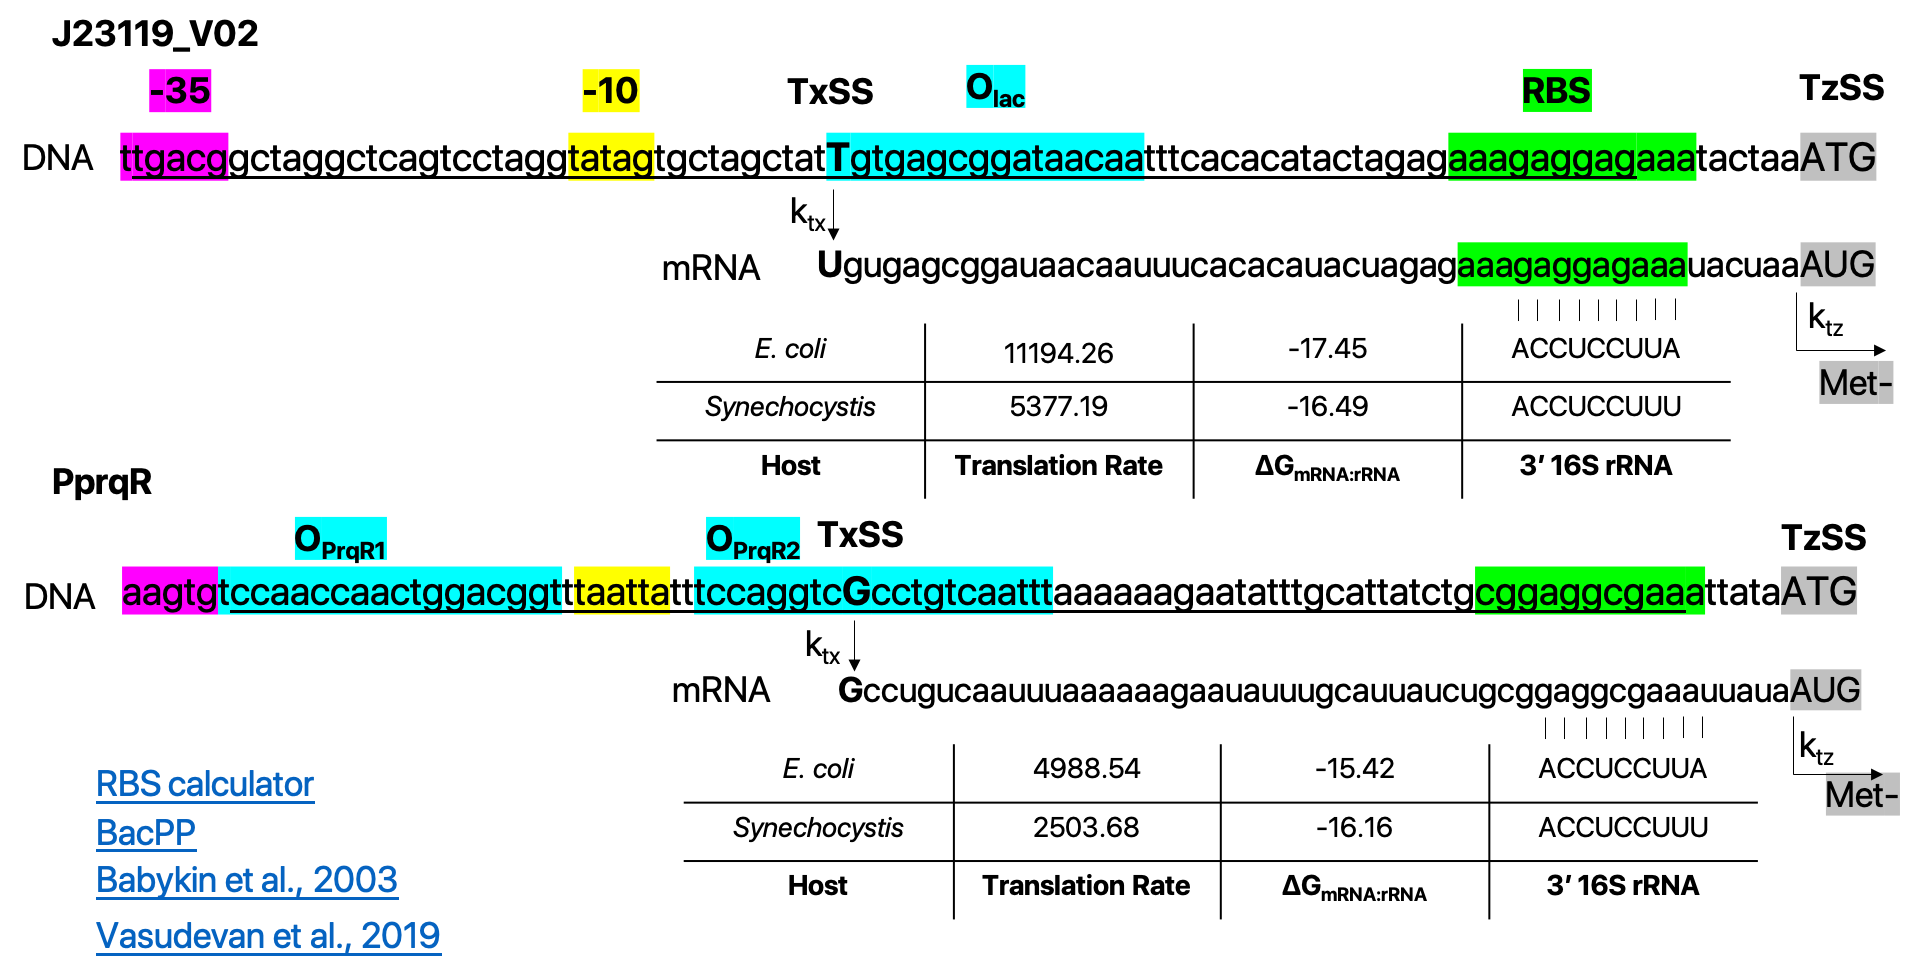
\includegraphics[width=\hsize]{figs/promoters.png}
    \caption{Comparison of the $P_{prqR}$ and the consensus J23119 promoter.}
    \label{fig:promoteranal}
\end{figure}

Cyanobacterial promoters can be categorised into three groups based on their sequences and which sigma factors recognise them. Type I promoters (recognised by $\sigma$70) contain both a −10 element (consensus 5’-TATAAT-3’) and a −35 element (consensus 5’-TTGACA-3’). Type II promoters contain the −10 element but lack a −35 element, instead containing operator sites bound by transcription factors. Type III promoters lack −10 or −35 elements and generally respond to various stresses through binding of type III sigma factors \citep{Gordon2018}.
Bioinformatic analysis of the $P_{prqR}$ promoter suggested that this promoter might be a type II promoter. In fact it contains a −10 element but the sequence at the −35 location is quite dissimilar to the -35 consensus (5’-TTGACA-3’), and instead contains two operator sites recognised by its repressor PrqR.

After this analysis, the annotated P$_{prqR}$ promoter sequence was assembled from annealing and extension of a pair of oligos (P58 and P59 in Table \ref{table:primers}) with overhangs compatible with the level 0 promoters acceptor.
This sequence was cloned upstream of the fluorescent protein eYFP. A positive control was constructed by replacing the P$_{prqR}$ with the J23119 consensus promoter. Terminators (T$_{clpPX}$) were added at the 3' end. 
The protein eYFP was chosen because of its fluorescent signal orthogonal to to the endogenous background fluorescence of \textit{Synechocystis sp.} PCC 6803 (Fig. \ref{fig:fluo}).

\begin{figure}[H]
    \centering
    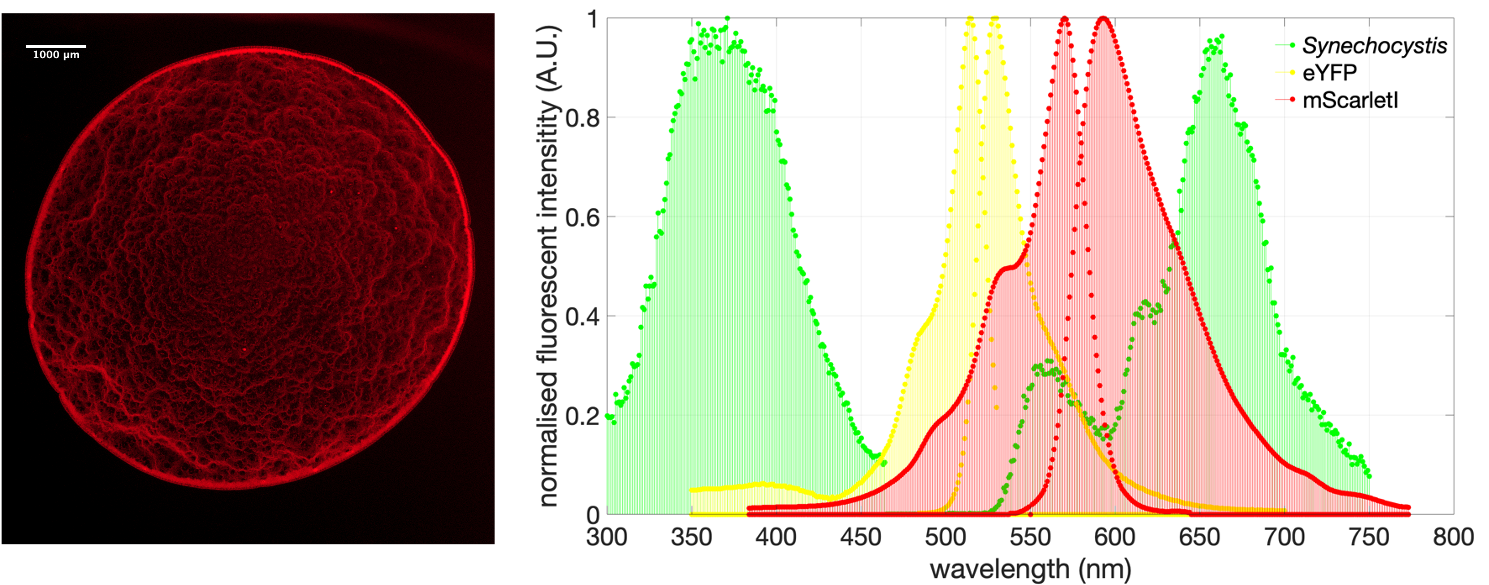
\includegraphics[width=\hsize]{figs/fspectracells.png}
    \caption{On the left: A colony of $\approx$ 4 million WT \textit{Synechocystis sp.} cells visualised under a fluorescence microscope ($\lambda_{em} = 667 nm$). The red signal is the endogenous fluorescence emitted by photosynthetic components (e.g. chlorophylls). On the right: fluorescence spectra of whole cells overlayed with those of the fluorescent reporters eYFP (yellow) and mScarlet-I.}
    \label{fig:fluo}
\end{figure}

\section{Mathematical Modelling of PrqR Dynamics}

The synthetic negative feedback network displayed by the prqRA operon was formalised using mathematical modelling in MATLAB R2019b. Regulation at both the transcriptional (repressor-promoter) and translational levels was modelled using a simple system of ordinary differential equations (ODE) commonly used to predict expression kinetics of synthetic gene circuits.
The autorepressor was simulated using a two-state model similar to previously described models of the TetR autorepressor (\citealt{Braun}; \citealt{Kelly2018}). The aim of this modelling is to predict the fluorescence output from the reporter plasmids constructed in this study depending on the concentration of redox-mediator. In one direction (theory $\rightarrow$ experiments), these results can help to identify suitable ranges of concentration of redox mediators to capture the sigmoidal fluorescence output characteristic of inducible promoters. In the other direction (experiments $\rightarrow$ theory), using this theoretical framework it would be possible to estimate the concentration of ligand effector present in the cell given the fluorescence output quantified from the experiments.




\begin{figure}[H]
    \centering
    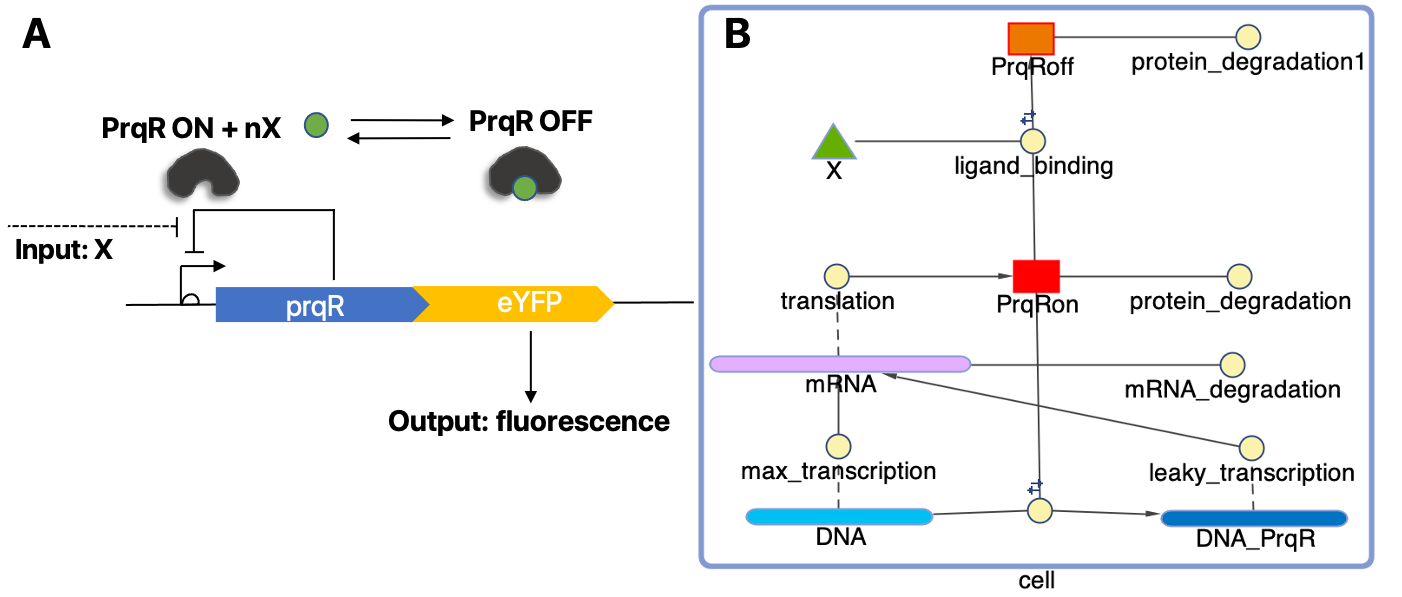
\includegraphics[width=\hsize]{figs/modelling.png}
    \caption{Schematic overview of a simple ODE model to simulate dynamics of prqRA operon. The PrqR repressor is an autorepressor of its own P$_{prqR}$ promoter. It has been assumed that the PrqR repressor behaves as other repressor in the tetR-like family. These transcriptional regulators generally exist in two states (ON or OFF) depending on the presence of ligand molecules. In the ON state, they represses transcription from their cis-regulatory sequences (e.g. prqR and eYFP in this case). Binding with ligand X induces a conformational change in the DNA-binding domain of the repressor, resulting in its inactivation (OFF) and consequent transcription of prqR and eYFP genes.}
\end{figure}

\subsection{Modelling Gene Expression}
Gene expression dynamics for the PrqR-YFP device is modelled with a simple system of kinetic reactions depending on two states: the concentration of mRNA (r) and protein (R). The underlying biochemical reactions (transcription, translation, degradation) can be expressed as:

\begin{equation}
\begin{gathered}    
    \emptyset \xrightarrow{k_{tx}} r \xrightarrow{d} \emptyset\\
    r \xrightarrow{k_{tz}} r + R\\ 
    R \xrightarrow{D} \emptyset
\end{gathered}
\end{equation}
Where $\Theta$ indicate empty sets (genes, degradation), $k_{tx}$is the apparent transcription rate, d is the mRNA degradation rate, $k_{tz}$ is the translation rate and D is the protein degradation rate. These reactions are described by two sets of ODEs:

\begin{equation}
\label{eq:transcription1}
    \frac{\delta r}{\delta t} = k_{tx}r - dr
\end{equation}

\begin{equation}
    \frac{\delta R}{\delta t} = k_{tz}r - DR
\end{equation}

\subsection{Repressor and Ligand Binding}
The binding between repressor and ligand is modelled as a second-order kinetic reaction. The DNA-bound active repressor, $R_{on}$, reacts with ligand X to form the inactive form of the repressor-ligand complex, $R_{off}$:
\begin{equation}
   R_{on} + nX \stackrel[k_{r}]{k_{f}}{\leftrightarrows} R_{off} 
\end{equation}
where n is the number of ligand binding sites in R,  $k_{f}$ and $k_{r}$ are the forward and reverse reaction rates. The rate of appearance of the repressor-ligand complex can then be described by the following ODE

\begin{equation}
\label{eq:ligandbinding}
    \frac{R_{off}}{dt} = k_{f}[R_{on}][X]^{n} - k_{r}[R_{off}] 
\end{equation}

If $[R_{off}]$ is initially zero, the concentrations will shift until the forward reaction rate is equal to the reverse reaction rate, such that the concentrations no longer vary with time. At this equilibrium point, the concentration of the complex won’t vary with time. Therefore equating Equation \ref{eq:ligandbinding} to 0 and after some algebraic rearrangement, the fractions of bound repressor molecules as a function of ligand concentration are described by the following Hill equation:

\begin{equation}
\label{eq:Hill}
    \Theta = \frac{Bound [PrqR]}{Total [PrqR]} =  \frac{[R_{off}]}{[R_{on}] + [X]^{n}}
\end{equation}

Therefore multiplying the total PrqR concentration, R, with the fraction of unbound molecules (1-$\Theta$) enables to calculate the concentration of active (DNA-bound) repressors at steady state:

\begin{equation}
\label{eq:Ron}
	R_{on} = R\cdot(1-\Theta) = R\cdot(1 - \frac{[X]^n}{Kd_{x} + [X]^n})
\end{equation}

Where  Kd$_{x}$  is the apparent dissociation constant, defined as the ratio of the dissociation rate constant ($k_{r}$) and the association rate constant ($k_{f}$) such that:

\begin{equation}
	Kd_{x} = \frac{k_{r}}{k_{f}} = \frac{[R_{on}][X]^n}{[R_{off}]}
\end{equation}

\subsection{Transcription as a Function of Active Repressor}
Equation \ref{eq:transcription1} describes the rate of transcription from the P$_{prqR}$ promoter but assumes that the promoter is very strong, such that all promoters were bound. However, in the case of prqR-mediated autorepression, we need to account for the amound of promoter sites bound by the repressor. It is assumed that all the repressors unbound by the ligand will bind to the promoters and vice versa.  Using the hill equation (Equation \ref{eq:Hill}), it is possible to describe the transcription from the P$_{prqR}$ promoter as a function of the concentration of active repressors, with the generic equation of the form:

\begin{equation}
\label{eq:transrep2}
    \frac{\delta r}{\delta t} = k_{tx} \cdot (1 - \frac{[R_{on}]^{N}}{K_D + [R_{on}]^{N}}) = \frac{k_{tx}}{1 + \frac{[R_{on}]^N}{K_D}}
\end{equation}

Additionally, even when fully bound, the promoter is still able to transcribe the downstream gene, but at a reduced rate. This is described as leaky transcription. The maximum transcription rate, $K_{tx}$ is therefore redefined as $\alpha$ + $\alpha_{0}$ in the presence of no repressors bound to the promoter and $\alpha_{0}$ when saturated with repressor R. The change in concentration of mRNA over time as a function of the repressor bound to the promoters can be then rewritten as:
    
\begin{equation}
    \frac{\delta r}{\delta t} = \frac{\alpha}{1 + \frac{[R_{on}]^{N}}{K_D}} + \alpha_{0}
\end{equation}

\subsection{Final System of ODEs}
By substituting the concentration of active repressor calculated in Equation \ref{eq:Ron} with $R_{on}$ of Equation \ref{eq:transrep2}, results in the final ODEs describing transcription of r as a function of ligand concentration: 
\begin{equation}
\label{eq:transcrtiptionrepress}
    \frac{\delta r}{\delta t} = \frac{\alpha}{1 + \frac{(R\cdot(1 - \frac{[X]^n}{Kd_{x} + [X]^n}))^{N}}{K_D}} + \alpha_{0} - dr
\end{equation}

The translation of r into R is given by Equation \ref{eq:translationtot}, which describes the change in protein concentration, R, over time as a function of the translation and degradation of mRNA,r.
\begin{equation}
\label{eq:translationtot}
    \frac{\delta R}{\delta t} = k_{tz}r - DR
\end{equation}


\subsection{Deterministic Simulation}
Equations \ref{eq:transcrtiptionrepress} and \ref{eq:translationtot} have been solved numerically using Matlab ode45 solver. The parameters used to run the simulation have been taken from biologically similar systems and are listed in Table \ref{table:params}. Future experimental efforts will also involve the quantification of some of these parameters.

\begin{table}[H]
\centering
\begin{tabular}{l|l|l|l|l}
\textbf{} & \textbf{Description} & \textbf{Value} & \textbf{Unit} & \textbf{Reference} \\ \hline
$\alpha$ & transcription rate of tetR-GFP gene from Ptet & 0.085 & nM $s^{-1}$ & \cite{Braun}\\ \hline
$\alpha_{0}$ & transcription leak rate of tetR-GFP gene from Ptet & 0.05 & nM $s^{-1}$ & \cite{Kelly2018} \\ \hline
d & mRNA degradation rate  & 4.1 $\cdot$ 10$^{−3}$ & s$^{-1}$  & \cite{Kelly2018}  \\ \hline
D & protein degradation rate & 3.9 $\cdot$ 10$^{−4}$ & s$^{-1}$  & \cite{Kelly2018}   \\ \hline
$k_{tz}$ & translation rate from from Ptet & 0.0154   & $s^{-1}$  & \cite{Kelly2018}  \\
\end{tabular}
\caption{List of parameters used utilised to simulate the system of ODEs}
\label{table:params}
\end{table}

As shown in Figure \ref{fig:modelgraphs} (on the left), the model predicts that the higher the concentration of inducer, the higher the steady-state fluorescence intensity. By plotting the steady state fluorescence as a function of ligand concentration, the model also predicts a sygmoidal dose response to the logarithm of ligand concentration. This is characteristic of a double-negative feedback with cooperativity \cite{Kelly2018}. The cooperativity parameter (the Hill coefficient n) determines the steepness of the response and can be fitted with experimental data to estimate the number of repressor monomers binding cooperatively to the promoter. These results have been simulated with parameters for the TetR repressor and tetracycline as the inducer. However, in the future, these parameters will be adapted to the ones for the redox-mediator tested experimentally (e.g. methyl viologen, pyocyanin etc...). The reporter devices will be characterised using serial dilutions of a range of different putative inducers. If the experimental data for a given inducer fit with the theoretical predictions of double-negative feedback, this would suggest that the inducer under study is a potential ligand to PrqR.

\begin{figure}[H]
    \centering
    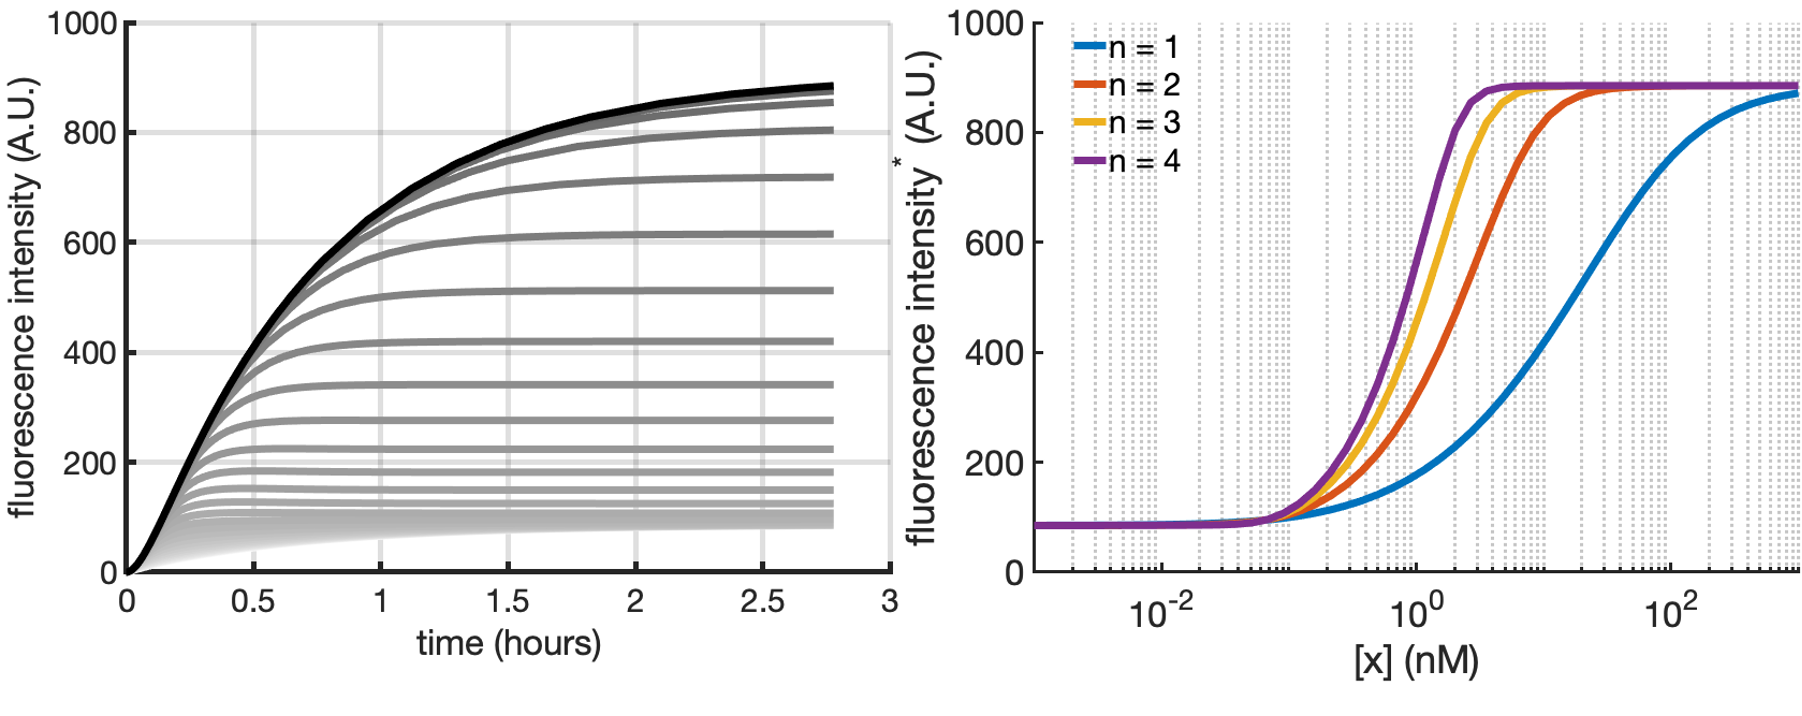
\includegraphics[width=\hsize]{figs/simulations.png}
    \caption{Numerical simulations of the system of ODEs describing the dynamics of PrqR regulation. On the left:eYFP fluorescence as a function of time for increasing concentrations of putative inducer X (increasing shades of grey). On the right: steady-state fluorescence response as a function of the logarithm of the inducer concentration. Lines of different colours indicate simulations with different Hill coefficients according to legend in the top left corner.}
    \label{fig:modelgraphs}
    \end{figure}


\end{document}
